\documentclass[twoside,a4paper]{refart}

\usepackage[utf8]{inputenc}
\usepackage{ae}
\usepackage[english]{babel}
\usepackage{csquotes}
\usepackage{hyperref}
\usepackage{xcolor}
\usepackage{amsmath}
\usepackage{amssymb}
\usepackage{amsthm}
\usepackage{dirtree}
\usepackage{booktabs}
\usepackage{tikz}
\usetikzlibrary{positioning,shapes,shadows,arrows,matrix,backgrounds}
\newcommand{\stencilpt}[4][]{\node[circle,fill,draw,inner sep=1.5pt,label={above:#4},#1] at (#2) (#3) {}}

\usepackage{array,lipsum}

\newenvironment{fulltable}[1][tbp]
{\begin{table}[#1]%
		\hspace*{-\leftmarginwidth}%
		\begin{minipage}{\fullwidth}}
		{\end{minipage}\end{table}}

\newenvironment{fullfigure}[1][tbp]
{\begin{figure}[#1]%
		\hspace*{-\leftmarginwidth}%
		\begin{minipage}{\fullwidth}}
		{\end{minipage}\end{figure}}

\theoremstyle{definition}
\newtheorem{exmp}{Example}

\title{PSBLAS-KINSOL interface\thanks{Work supported by the EC under the Horizon 2020 Project ``Energy oriented Centre of Excellence for computing applications'' (EoCoE II), Project ID: 824158}}
\author{Istituto per le Applicazioni del Calcolo ``M. Picone'',\\
	Consiglio Nazionale delle Ricerche \\
	Pasqua D'Ambra \\
	Fabio Durastante \\
	Salvatore Filippone \\
	PSBLAS development --- Kinsol Interface Version 1}
\date{\today}
\emergencystretch1em

\setcounter{tocdepth}{2}
\settextfraction{0.7}

\definecolor{mGreen}{rgb}{0,0.6,0}
\definecolor{mGray}{rgb}{0.5,0.5,0.5}
\definecolor{mPurple}{rgb}{0.58,0,0.82}
\definecolor{blue(ncs)}{rgb}{0.0, 0.53, 0.74}
\definecolor{sunGreen}{HTML}{70ad47}
\definecolor{sunCyan}{HTML}{dae3f3}
\definecolor{sunBlue}{HTML}{8faadc}
\usepackage{listings}
\lstdefinestyle{CStyle}{
	commentstyle=\color{mGreen},
	keywordstyle=\color{magenta},
	numberstyle=\tiny\color{mGray},
	stringstyle=\color{mPurple},
	basicstyle=\footnotesize,
	breakatwhitespace=false,
	breaklines=true,
	captionpos=b,
	keepspaces=true,
%	numbers=left,
	numbersep=5pt,
	showspaces=false,
	showstringspaces=false,
	showtabs=false,
	tabsize=2,
	language=C,
	morekeywords={N_Vector,SUNMatrix,sunindextype,psb_i_t,psb_c_descriptor,psb_c_dvector,booleantype,psb_l_t,realtype,psb_c_SolverOptions,SUNLinearSolver,SUNLinearSolver_Type,MPI_IN_PLACE,MPI_LONG,MPI_SUM,NULL,psb_d_t,SUNTRUE,SUNFALSE,free,malloc,MPI_Comm,printf,fprintf,SUNDIALS_NVEC_CUSTOM,bool},
	emph={%  
		psb_c_info,psb_c_init,psb_cdall,psb_c_cdall_vl,psb_c_cdall_nl,psb_c_abort,psb_c_new_descriptor,%
		psb_c_set_index_base,psb_c_dfree,psb_c_exit,psb_c_cdall_vg,psb_c_cdasb,psb_c_DefaultSolverOptions,%
		MPI_Comm_f2c,MPI_Allreduce,psb_c_barrier,psb_c_l_idx2ijk,psb_c_l_ijk2idx,psb_c_dgeins,%
		psb_c_cd_get_global_indices,psb_c_cd_get_local_rows%
		},emphstyle={\color{blue(ncs)}}
}

\usepackage[backend=biber,sorting=nty,sortcites=true]{biblatex}
\bibliography{bibliography}

\begin{document}
	\maketitle
	
	\tableofcontents
	\newpage
	
	
	\section{SUNDIALS KINSOL: Newton--Krylov Solvers}
	
	The original SUNDIALS library is a SUite of Nonlinear and DIfferential/ALgebraic equation Solvers.  It consists of the following six solvers:
	\begin{itemize}
		\item CVODE, solves initial value problems for ordinary differential equation (ODE) systems;
		\item CVODES, solves ODE systems and includes sensitivity analysis capabilities (forward and adjoint);
		\item ARKODE, solves initial value ODE problems with additive Runge-Kutta methods, include support for IMEX methods;
		\item IDA, solves initial value problems for differential-algebraic equation (DAE) systems;
		\item IDAS, solves DAE systems and includes sensitivity analysis capabilities (forward and adjoint);
		\item KINSOL, solves nonlinear algebraic systems.
	\end{itemize}
	
	The numerical operations performed in these codes are operations on vectors and matrices, and the codes provides both custom implementation and interfaces to these vector operations. What we provide here is a particular interface for such operations to the linear algebra operations provided by the Parallel Sparse BLAS (PSBLAS) library~\cite{filippone2000psblas,filippone2012object}; see the whole structure of the library in Figure~\ref{fig:software_structure}.

	\begin{fullfigure}[htpp]
	\centering
	\tikzstyle{library}=[rectangle, draw=black, rounded corners, fill=yellow!40, drop shadow,
	text centered, anchor=north, text=black, text width=2.5cm]
	\tikzstyle{api}=[rectangle, draw=black, fill=sunGreen, drop shadow,
	text centered, anchor=north, text=black, text width=4cm]
	\begin{tikzpicture}[scale=0.73, transform shape]
		\node (SUNDIALS) [library]{ SUNDIALS };
		\node (center) [below=of SUNDIALS] {};
		\node (ARKODE) [library, left=of center]{ ARKODE };
		\node (CVODES) [library, left=of ARKODE]{ CVODES };
		\node (CVODE) [library, left=of CVODES]{ CVODE };		
		\node (IDA) [library, right=of ARKODE]{ IDA };
		\node (IDAS) [library, right=of IDA]{ IDAS };
		\node (KINSOL) [library, right=of IDAS]{ KINSOL };
		\draw (SUNDIALS.south) -- ([yshift=0.5cm, xshift=0cm]center.north);
		\draw[->] ([yshift=0.5cm, xshift=0cm]center.north) -| (CVODE.north);
		\draw[->] ([yshift=0.5cm, xshift=0cm]center.north) -| (CVODES.north);
		\draw[->] ([yshift=0.5cm, xshift=0cm]center.north) -| (ARKODE.north);
		\draw[->] ([yshift=0.5cm, xshift=0cm]center.north) -| (IDA.north);
		\draw[->] ([yshift=0.5cm, xshift=0cm]center.north) -| (IDAS.north);
		\draw[->] ([yshift=0.5cm, xshift=0cm]center.north) -| (KINSOL.north);
		\node (center2) [text width=0cm,below=of ARKODE] {};
		\draw[-] ([yshift=-0cm, xshift=0cm]CVODE.south) |- ([yshift=0.5cm, xshift=0cm]center2.north);
		\draw[-] ([yshift=-0cm, xshift=0cm]CVODES.south) |- ([yshift=0.5cm, xshift=0cm]center2.north);
		\draw[-] ([yshift=-0cm, xshift=0cm]ARKODE.south) |- ([yshift=0.5cm, xshift=0cm]center2.north);
		\draw[-] ([yshift=-0cm, xshift=0cm]IDA.south) |- ([yshift=0.5cm, xshift=0cm]center2.north);
		\draw[-] ([yshift=-0cm, xshift=0cm]IDAS.south) |- ([yshift=0.5cm, xshift=0cm]center2.north);
		\draw[-] ([yshift=-0cm, xshift=0cm]KINSOL.south) |- ([yshift=0.5cm, xshift=0cm]center2.north);
		\node (SUNMATRIX) [api,text width=3.5cm,left=of center2,xshift=1.2cm,yshift=-0.3cm] {SUNMATRIX API};
		\node (NVECTOR) [api,left=of SUNMATRIX] {NVECTOR API};
		\node (SUNLINEARSOLVER) [api,text width=4.5cm,right=of center2,yshift=-0.3cm] {SUNLINEARSOLVER API};
		\node (SUNNONLINEARSOLVER) [api,text width=5.5cm,right=of SUNLINEARSOLVER] {SUNNONLINEARSOLVER API};
		\draw[->] ([yshift=0.5cm, xshift=0cm]center2.south) -| ([yshift=0cm, xshift=0cm]SUNMATRIX.north);
		\draw[->] ([yshift=0.5cm, xshift=0cm]center2.south) -| ([yshift=0cm, xshift=0cm]NVECTOR.north);
		\draw[->] ([yshift=0.5cm, xshift=0cm]center2.south) -| ([yshift=0cm, xshift=0cm]SUNLINEARSOLVER.north);
		\draw[->] ([yshift=0.5cm, xshift=0cm]center2.south) -| ([yshift=0cm, xshift=0cm]SUNNONLINEARSOLVER.north);
		\draw[->] ([yshift=-0.65cm, xshift=-2cm]center.south) -- ([yshift=0.45cm, xshift=0.5cm]center2.south);
		\matrix (vectormodules)[matrix of nodes,nodes={rectangle, rounded corners, draw=black, fill=gray!20,
			text centered, anchor=north, text=black, text width=1.3cm,font={\tiny}},column sep=2mm, row sep=1mm,below=of NVECTOR]{
			SERIAL & PARALLEL (MPI) \\
			OPENMP & PTHREADS \\
			PARHYP (HYPRE) & PETSC \\
			CUDA & RAJA \\
			MPI + CUDA & MPI + RAJA \\
			OPENMP & |[rectangle,draw,fill=red!70]| PSBLAS \\
		};
		\node[font=\scriptsize,anchor=south] (vectormodtitle) at (vectormodules.north) {\textbf{VECTOR MODULES}};
		\matrix (matrixmodules)[matrix of nodes,nodes={rectangle, rounded corners, draw=black, fill=gray!20,
		text centered, anchor=north, text=black, text width=1.3cm,font={\tiny}},column sep=2mm, row sep=1mm,below=of SUNMATRIX]{
		DENSE \\
		BAND \\
		SPARSE \\
		|[rectangle,draw,fill=red!70]|PSBLAS \\
		};
		\node[font=\scriptsize,anchor=south] (matrixmodtitle) at (matrixmodules.north) {\textbf{MATRIX MODULES}};
		\matrix (lsmodules)[matrix of nodes,nodes={rectangle, rounded corners, draw=black, fill=gray!20,
			text centered, anchor=north, text=black, text width=1.5cm,font={\tiny}},column sep=2mm, row sep=1mm,rectangle,fill=sunBlue,draw=black,below=of SUNLINEARSOLVER,yshift=-0.45cm]{
			DENSE & BAND \\
			LAPACK DENSE & LAPACK BAND \\
			KLU & SUPERLU\_MT \\
			|[rectangle,draw,fill=red!70]| PSBLAS MLD2P4 & \\
		};
		\node[font=\scriptsize,anchor=south] (overtitle) at (lsmodules.north) {\textbf{MATRIX BASED}};
		\node[font=\scriptsize,anchor=south] (linearsolmodtitle) at (overtitle.north) {\textbf{LINEAR SOLVER MODULES}};
		\node[font=\scriptsize,anchor=south] (undertitle) at ([yshift=-0.6cm]lsmodules.south) {\textbf{MATRIX-FREE}};
		\matrix (lsmodules2)[matrix of nodes,nodes={rectangle, rounded corners, draw=black, fill=gray!20,
			text centered, anchor=north, text=black, text width=1.5cm,font={\tiny}},column sep=2mm, row sep=1mm,rectangle,fill=sunBlue,draw=black,below=of undertitle,yshift=1cm]{
			SPBCG & SPGMR \\
			SPFGMR & SPTFQMR \\
			PCG & \\
		};
		\matrix (lsmodules3)[matrix of nodes,nodes={rectangle, rounded corners, draw=black, fill=gray!20,
			text centered, anchor=north, text=black, text width=1.5cm,font={\tiny}},column sep=2mm, row sep=1mm,rectangle,below=of SUNNONLINEARSOLVER]{
			NEWTON \\
			FIXED POINT \\
		};
		\node[font=\scriptsize,anchor=south] (nonlinearsolmodtitle) at (lsmodules3.north) {\textbf{NONLINEAR SOLVER MODULES}};
		\draw[->] (NVECTOR.south) -- (vectormodtitle.north);
		\draw[->] (SUNMATRIX.south) -- (matrixmodtitle.north);
		\draw[->] (SUNLINEARSOLVER.south) -- (linearsolmodtitle.north);
		\draw[->] (SUNNONLINEARSOLVER.south) -- (nonlinearsolmodtitle.north);
		\begin{scope}[on background layer]
		\draw[fill=sunCyan,draw=black] ([xshift=-0.8cm]vectormodtitle.north west) rectangle (vectormodules.south east);
		\draw[fill=sunCyan,draw=black] (matrixmodtitle.north west) rectangle ([xshift=0.4cm]matrixmodules.south east);
		\draw[fill=sunCyan,draw=black] (matrixmodtitle.north west) rectangle ([xshift=0.4cm]matrixmodules.south east);
		\draw[fill=sunCyan,draw=black] ([xshift=-0.65cm,yshift=0cm]linearsolmodtitle.north west) rectangle ([xshift=0.2cm,yshift=-0.2cm]lsmodules2.south east);
		\draw[fill=sunCyan,draw=black] (nonlinearsolmodtitle.north west) rectangle ([xshift=1.3cm,yshift=-0.1cm]lsmodules3.south east);
		\end{scope}
	\end{tikzpicture}
	\caption{High-level diagram of the sundials suite, the additions presented here are highlighted in red.}\label{fig:software_structure}
	\end{fullfigure}

	Furthermore, many of the solvers included in SUNDIALS require the solution of linear systems of algebraic equations. For this task we provide a suite of parallel matrix--based Krylov solvers and preconditioners from the Multilevel Domain Decomposition Parallel Preconditioners Packages based on PSBLAS (MLD2P4)~\cite{MR2738234}.

	Our main objective is enabling the solution of nonlinear algebraic systems $F(\mathbf{x}) = 0$, for $\mathbf{x} \in \mathbf{R}^n$, by means of Newton--Krylov solvers. The rest of this documentation presents the extension of the KINSOL package~\cite{kinsolguide} NVECTOR, SUNMATRIX and SUNLINSOL API with the functionalities offered by PSBLAS/MLD2P4.
		
	\subsection{How to install}
	
	The first step for using these interfaces is to have a working version of both the PSBLAS and MLD2P4 library. The installation chain is therefore the following. As a first step you need to have all the auxiliary packages needed/suggested for the PSBLAS library, e.g., a local implementation of the BLAS library, the LAPACK library, METIS and AMD libraries. Then the development version from
	\begin{center}
		\url{https://github.com/sfilippone/psblas3}
	\end{center}
	can be cloned, and installed; please refer to its manual for the complete details on the install procedure. \attention If you want to compile KINSOL as a dynamic library it is necessary to pass the \lstinline|-fPic -ldl| flags to the PSBLAS configure. The next packages that you need to install is the package of extensions for PSBLAS from
	\begin{center}
		\url{https://github.com/sfilippone/psblas3-ext}.
	\end{center}
	The next step is then to install the suite of preconditioners, i.e., the MLD2P4 package. This packages has on its own a certain number of interfaces to other scientific libraries that are used to perform certain operation within it, e.g., the MUMPS, UMFPACK, SuperLU and SuperLUDist libraries. After the needed auxiliary packages have been installed, you need to install the library (again from the development branch) from
	\begin{center}
		\url{https://github.com/sfilippone/mld2p4-2}.
	\end{center}

	After all these operation have been completed, you can finally install the KINSOL-PSBLAS library from
	\begin{center}
		\url{https://github.com/Cirdans-Home/kinsol-psblas}.
	\end{center}
	The installation of this library uses CMake and requires the user to provide the location of the installation directories of PSBLAS, PSBLAS-EXT and MLD2P4-2 libraries.

		
	\section{The logic behind a PSBLAS instrumented application}
	
\marginlabel{
\textit{Library structure}
\begin{minipage}{0.9\textwidth}
\dirtree{%
 .1 kinsol-psblas.
 .2 config.
 .2 doc.
 .2 examples.
 .2 include.
 .2 src.
 .2 test.
}
\end{minipage}
}	The main aim of the PSBLAS library is the parallel implementation of iterative solvers
	for sparse linear systems,
	\begin{equation}\label{eq:linear_system}
		A \mathbf{x} = \mathbf{b}, \qquad A \in \mathbb{K}^{n \times n}, \qquad \mathbb{K} = \mathbb{R}, \mathbb{C},
	\end{equation}
	through the distributed memory paradigm operating with message
	passing. The library includes all the needed routines for this task, e.g, functions for multiplying sparse matrices by dense matrices, for solving block diagonal systems with triangular diagonal entries or for preprocessing sparse matrices.
	
	The pivotal choice to be made in this setting regards the distribution of the coefficient matrix $A$ for the linear system~\eqref{eq:linear_system}. In PSBLAS this choice is based on the \textbf{owner computes rule}: \marginlabel{\textbf{Owner computes rule}} each unknown is assigned to a process that will  own the corresponding row in the coefficient matrix and
	will  carry out all related computations.
	
	If $A$ is obtained from the discretization of a Partial Differential Equation (PDE), this allocation strategy is equivalent to the choice of a partition of the mesh into {\em
		sub-domains}.
	
	\attention PSBLAS supports \emph{any} distribution that keeps together
	the coefficients of each matrix row there are \textbf{no other} constraints on
	the variable assignment.
	
	Any PSBLAS application will always start with the construction of the parallel environment, i.e., of an MPI (virtual) parallel machine, that we call here context by means of the \lstinline[style=CStyle]|psb_c_init| function~as
\begin{lstlisting}[style=CStyle]
psb_i_t ictxt, iam, np;
ictxt = psb_c_init();
psb_c_info(ictxt,&iam,&np);
\end{lstlisting}
	that creates a parallel environment on \lstinline[style=CStyle]|np| processors $0,\ldots,\lstinline[style=CStyle]|np|-1$, of which we are process \lstinline[style=CStyle]|iam|.
	
\begin{description}
	\item[\fbox{psb\_c\_init}] this subroutine initializes the PSBLAS parallel environment, defining a virtual parallel machine, the value \texttt{ictxt} in out is the communication context identifying the virtual parallel machine.
	This is always a duplicate of \texttt{basectxt}, so that library communications are completely separated from other communication operations
	
	\marginlabel{Prototype} \lstinline[style=CStyle]|psb_i_t psb_c_init()|
	
	\item[\fbox{psb\_c\_info}] this subroutine returns information about the PSBLAS parallel environment, defining a virtual parallel machine that is identified by the value \texttt{ictxt}. The values on return are the identifier of current process in the PSBLAS virtual parallel machine (\texttt{iam}), and the number of processes in the PSBLAS virtual parallel machine~(\texttt{np})
	
	\marginlabel{Prototype} \lstinline[style=CStyle]|psb_i_t psb_c_info(psb_i_t ictxt,psb_i_t *iam,psb_i_t *np)|
	
\end{description}	
	
	The next step is represented by the need of subdividing the index space among processes, and this creates a mapping from the ``global'' numbering $1,\ldots,n$ to a ``local'' numbering
	in each process. This means that each process $i$ will own a certain subset
	$1,\ldots,n_{\hbox{row}_i}$, each element of which corresponds to a certain element of $1\dots n$.
	
	Therefore, after the initialization the first step is to establish an index space, and
	this is done with a call to one of the variants of the \lstinline[style=CStyle]|psb_cdall| function to allocate a descriptor object \lstinline[style=CStyle]|psb_c_descriptor|:
\begin{description}
	\item[\fbox{\texttt{psb\_c\_cdall\_vg}}] the association between an index and a process is specified via an integer vector \lstinline[style=CStyle]|vg[]|, each index $i \in \{1,\ldots,\lstinline[style=CStyle]|ng|\}$ is assigned to process \lstinline[style=CStyle]|vg[i]|. The vector \lstinline[style=CStyle]|vg[]| must be identical on all calling processes, and its entries have the ranges $(0,\ldots,\lstinline[style=CStyle]|np|-1)$ or
	$(1,\ldots,\lstinline[style=CStyle]|np|)$ according to the fact that \lstinline[style=CStyle]|psb_c_set_index_base(0)| or \lstinline[style=CStyle]|psb_c_set_index_base(1)| has been called at the beginning. The size \lstinline[style=CStyle]|ng| is specified one can chose to use the entire
	vector \lstinline[style=CStyle]|vg[]|, thus having \lstinline[style=CStyle]|vg[ng]|.
	
	\marginlabel{Prototype} \lstinline[style=CStyle]|psb_c_cdall_vg(psb_l_t ng,psb_i_t *vg,psb_i_t ictxt,psb_c_descriptor *cdh)|
	\item[\fbox{\texttt{psb\_c\_cdall\_vl}}] the association is done by specifying the list of indices \lstinline[style=CStyle]|vl[nl]| assigned to
	the current process; thus, the global problem size \lstinline[style=CStyle]|nl| is given by
	the range of the aggregate of the individual vectors \lstinline[style=CStyle]|vl[]| specified in
	the calling processes. The subroutine will check how
	many times each entry in the global index space $(1,\ldots,\lstinline[style=CStyle]|nl|)$ is specified
	in the input lists \lstinline[style=CStyle]|vl[]|, therefore it allows for the presence of overlap in the
	input, and checks for the ``orphan'' indices.
	
	\marginlabel{Prototype} \lstinline[style=CStyle]|psb_c_cdall_vl(psb_i_t nl,psb_l_t *vl,psb_i_t ictxt,psb_c_descriptor *cdh)|
	\item[\fbox{\texttt{psb\_c\_cdall\_nl}}] produces a generalized block-row distribution of the number of indices belonging to the current process in which each process $i$ gets assigned
	a consecutive chunk of $nl$ global indices,
	
	\marginlabel{Prototype} \lstinline[style=CStyle]|psb_c_cdall_nl(psb_i_t nl,psb_i_t ictxt, psb_c_descriptor *cdh)|
\end{description}
	for the case of a simple minded block distribution, i.e., the index space is first numbered sequentially in a standard way, then the corresponding vector is distributed according to a block distribution directive.
	%The discretization ensures there are IDIM *internal* points in each direction.
	
\begin{exmp}\label{ex:the_example}
We consider as example the finite difference discretization of the following boundary value problem
\begin{equation}\label{eq:boundaryproblem}
	- \frac{b_1 \partial^2 u}{\partial x^2} - \frac{b_2 \partial^2 u}{\partial y^2} - \frac{b_3 \partial^2 u}{\partial z^2} + \frac{a_1 \partial u}{\partial x} + \frac{a_2 \partial u}{\partial y} + a_3 \frac{a_3 \partial u}{\partial z} = 0,
\end{equation}
for $(x,y,z) \in [0,1]^3$, with Dirichlet boundary conditions, on a uniform grid with \lstinline[style=CStyle]|idim| node per size. All the allocation procedure can be expressed as
\begin{lstlisting}[style=CStyle,caption="Example of allocation procedure for a 3D block data distribution",label=lst:example_of_allocation]
psb_c_descriptor *cdh;
psb_i_t idim,nb,nlr, nl;
psb_l_t i,ng, *vl, k;

cdh=psb_c_new_descriptor();
psb_c_set_index_base(0);

/* Simple minded BLOCK data distribution */
ng = ((psb_l_t) idim)*idim*idim;
nb = (ng+np-1)/np;
nl = nb;
if ( (ng -iam*nb) < nl) nl = ng -iam*nb;
fprintf(stderr,"%d: Input data %d %ld %d %d\n",iam,idim,ng,nb, nl);
if ((vl=malloc(nb*sizeof(psb_l_t)))==NULL) {
	fprintf(stderr,"On %d: malloc failure\n",iam);
	psb_c_abort(ictxt);
}
i = ((psb_l_t)iam) * nb;
for (k=0; k<nl; k++)
	vl[k] = i+k;
psb_c_cdall_vl(nl,vl,ictxt,cdh);
\end{lstlisting}
\end{exmp}

	Now that the initial distribution of the index space has been performed, we need to allocate  dense vectors and sparse matrices on such index space, and thus we define the complete topology of our computational problem. Since our task is to use the capabilities of SUNDIALS-KINSOL to solve for nonlinear problems, here lies the core of the interfacing between the two codes.

	Before the termination of the program, \textit{after} having freed/destroyed all the objects instantiated on the descriptor \texttt{cdh}, you need also to free the memory occupied by it, and the to terminate the parallel environment. This is achieved by means of the following routines.
	\begin{description}
		\item[\fbox{\texttt{psb\_c\_cdfree}}] frees a communication descriptor
		
		\marginlabel{Prototype} \lstinline[style=CStyle]|psb_i_t psb_c_cdfree(psb_c_descriptor *cdh)|
		
		\item[\fbox{\texttt{psb\_c\_exit}}] this subroutine exits from the PSBLAS parallel virtual machine, observe that this routine may be called even if a previous call to \lstinline[style=CStyle]|psb_info| has returned with \lstinline[style=CStyle]|iam=-1|.
		
		\marginlabel{Prototype} \lstinline[style=CStyle]|psb_i_t psb_c_exit(psb_i_t ictxt)|
		
		\item[\fbox{\texttt{psb\_c\_abort}}] this subroutine aborts computation on the parallel virtual machine, and can be used when error that needs the program to fail occurs.
		
		\marginlabel{Prototype} \lstinline[style=CStyle]|psb_i_t psb_c_abort(psb_i_t ictxt)| 		
		
	\end{description}


	
	In the next two Sections~\ref{sec:nvector}, and Section~\ref{sec:sunmatrix} we describe such encapsulation for dense vector, and sparse matrices. Then in Section~\ref{sec:sunlinsol} we describe the interfacing with the \textbf{linear solvers} and \textbf{preconditioners}

	Complete information on the PSBLAS data structures, and functions that are mentioned along the text can be found in~\cite{psblasguide}.
	
	
	\section{The NVECTOR\_PSBLAS implementation}\label{sec:nvector}
\marginlabel{
\textit{Library structure}
\begin{minipage}{0.9\textwidth}
\dirtree{%
 .1 kinsol-psblas.
 .2 config.
 .2 doc.
 .2 examples.
 .3 nvector.
 .4 psblas.
 .2 include.
 .3 nvector.
 .2 src.
 .3 nvector.
 .4 psblas.
 .2 test.
}
\end{minipage}
}	The NVECTOR\_PSBLAS implementation of the SUNDIALS NVECTOR module provides an interface to the PSBLAS code for handling distributed dense vectors.
	It defines the \emph{content} field of \texttt{N\_Vector} to be a structure containing the PSBLAS descriptor for the data distribution, a PSBLAS vector of double, and the PSBLAS communicator (context).
	
\begin{lstlisting}[style=CStyle]
struct _N_VectorContent_PSBLAS {
	booleantype own_data;  /*ownership of data*/
	psb_c_descriptor *cdh; /*descriptor for data distribution*/
	psb_c_dvector *pvec;   /*PSBLAS vector*/
	int ictxt;             /*PSBLAS communicator*/
};
\end{lstlisting}
	
	\attention All the vectors that have to interact needs to be instantiated on the same parallel context \lstinline[style=CStyle]|ictxt|, and on the same data distribution \lstinline[style=CStyle]|cdh|.
	
	
	The header file to include when using this module is \texttt{nvector\_psblas.h}. The installed module library to link to is \texttt{sundials\_nvecpsblas.lib} where \texttt{.lib} is typically \texttt{.so} for shared libraries and \texttt{.a} for static libraries.
	
	\subsection{NVECTOR\_PSBLAS accessor macros}
	
	The following macros are provided to access the content of a NVECTOR\_PSBLAS vector. The suffix \texttt{\_P} in the names denotes the fact that the data are in distributed memory.

\begin{lstlisting}[style=CStyle]
#define NV_CONTENT_P(v)   ((N_VectorContent_PSBLAS)(v->content))
#define NV_DESCRIPTOR_P(v)(NV_CONTENT_P(v)->cdh)
#define NV_OWN_DATA_P(v)  (NV_CONTENT_P(v)->own_data)
#define NV_PVEC_P(v)      (NV_CONTENT_P(v)->pvec)
#define NV_ICTXT_P(v)     (NV_CONTENT_P(v)->ictxt)
\end{lstlisting}

\marginlabel{\lstinline[style=CStyle]|NV_CONTENT_P(v)|} this macro gives access to the contents of the PSBLAS vector \texttt{N\_Vector}.

\marginlabel{\lstinline[style=CStyle]|NV_DESCRIPTOR_P(v),NV_OWN_DATA_P(v),NV_PVEC_P(v)|} these macros give instead individual access to the parts of the content of a PSBLAS parallel \texttt{N\_Vector}.

\marginlabel{\lstinline[style=CStyle]|NV_ICTXT_P(v)|} this macro provides the PSBLAS context used by the NVECTOR\_PSBLAS vectors.

\subsection{NVECTOR\_PSBLAS functions}

The NVECTOR\_PSBLAS implementation provides PSBLAS implementations of all the vectors operations listed in Tables~6.2, 6.3, and 6.4 of the original KINSOL library~\cite{kinsolguide}. Following the standard nomenclature of the SUNDIALS library, their names are obtained from the ones listed in Tables~6.2, 6.3, and 6.4 by appending the suffix \texttt{\_PSBLAS}. The NVECTOR\_PSBLAS implementation provides the following additional user--callable routine:

\begin{description}
	\item[\fbox{\texttt{N\_VAsb\_PSBLAS}}] This routine assemble the NVector after that all the elements have been inserted into it, i.e., after that all the calls to the \texttt{N\_VMake\_PSBLAS} routine have been completed. This is substantially a wrapper for the PSBLAS function \lstinline[style=CStyle]|psb_c_dgeasb|.

	\marginlabel{Prototype} \lstinline[style=CStyle]|void N_VAsb_PSBLAS(N_Vector v)|
\end{description}

\subsubsection{Description of the NVECTOR\_PSBLAS functions}

\begin{description}
	\item[\fbox{\texttt{N\_VNew\_PSBLAS}}] This function creates and allocates memory for a parallel vector
	on the PSBLAS context \lstinline[style=CStyle]|ictxt| with the communicator \lstinline[style=CStyle]|cdh|
	
	\marginlabel{Prototype} \lstinline[style=CStyle]|N_Vector N_VNew_PSBLAS(int ictxt, psb_c_descriptor *cdh)|
	
	\item[\fbox{\texttt{N\_VNewEmpty\_PSBLAS}}] This function creates a new PSBLAS vector with empty data array.
	
	\marginlabel{Prototype} \lstinline[style=CStyle]|N_Vector N_VNewEmpty_PSBLAS(int ictxt, psb_c_descriptor *cdh)|
	
	\item[\fbox{\texttt{N\_VMake\_PSBLAS}}] Function to create a PSBLAS \texttt{N\_Vector} with user data component. This function is substantially a wrapper for the PSBLAS function \lstinline[style=CStyle]|psb_c_dgeins|.
	
	\marginlabel{Prototype} \lstinline[style=CStyle]|N_Vector N_VMake_PSBLAS(int ictxt, psb_c_descriptor *cdh,psb_i_t m, psb_i_t *irow,double *val)|
	
	The PSBLAS context \lstinline[style=CStyle]|ictxt| with the communicator \lstinline[style=CStyle]|cdh| are the one defined for the whole programs, the integer \lstinline[style=CStyle]{m} is the number of rows in \lstinline[style=CStyle]{val[]} to be inserted, the array of integers \lstinline[style=CStyle]{irow} is the indices of the rows to be inserted. Specifically, row \lstinline[style=CStyle]|i| of \lstinline[style=CStyle]|val| will be inserted into the local row corresponding to the global index row index \lstinline[style=CStyle]|row[i]|.
	
	\attention This routine does not assemble the final vector. After the insertion of all the elements has been completed then the vector should be assembled by means of the \texttt{N\_VAsb\_PSBLAS} routine.
	
	\item[\fbox{\texttt{N\_VCloneVectorArray\_PSBLAS}}] This function creates an array of new parallel vectors (by cloning) an array of \lstinline[style=CStyle]|count| parallel vectors \lstinline[style=CStyle]|v|.
	
	\marginlabel{Prototype} \lstinline[style=CStyle]|N_Vector *N_VCloneVectorArray_PSBLAS(int count, N_Vector w)|
	
	\item[\fbox{\texttt{N\_VCloneVectorArrayEmpty\_PSBLAS}}] This function creates an array of \lstinline[style=CStyle]|count| new parallel vectors with empty data array on the same communicator and context of the vector \lstinline[style=CStyle]|w|.
	
	\marginlabel{Prototype} \lstinline[style=CStyle]|N_Vector *N_VCloneVectorArrayEmpty_PSBLAS(int count, N_Vector w)|
	
	\item[\fbox{\texttt{N\_VDestroyVectorArray\_PSBLAS}}] This function to frees an array of \lstinline[style=CStyle]|count| \texttt{N\_Vector}s created with \texttt{N\_VCloneVectorArray\_PSBLAS}
	
	\marginlabel{Prototype} \lstinline[style=CStyle]|void N_VDestroyVectorArray_PSBLAS(N_Vector *vs, int count)|
	
	\item[\fbox{\texttt{N\_VGetLength\_PSBLAS}}] This function returns the \emph{global} vector length, this is substantially a wrapper for the PSBLAS function \lstinline[style=CStyle]|psb_c_cd_get_global_rows|.
	
	\marginlabel{Prototype} \lstinline[style=CStyle]|sunindextype N_VGetLength_PSBLAS(N_Vector v)|
	
	\item[\fbox{\texttt{N\_VGetLocalLength\_PSBLAS}}] This function returns the \emph{local} vector length, this is substantially a wrapper for the PSBLAS function \lstinline[style=CStyle]|psb_c_cd_get_local_rows|.
	
	\marginlabel{Prototype} \lstinline[style=CStyle]|sunindextype N_VGetLocalLength_PSBLAS(N_Vector v)|
	
	\item[\fbox{\texttt{N\_VPrint\_PSBLAS}}] This function prints the local data in a parallel vector to \lstinline[style=CStyle]|stdout|.
	
	\marginlabel{Prototype} \lstinline[style=CStyle]|void N_VPrint_PSBLAS(N_Vector x)|
	
	\item[\fbox{\texttt{N\_VPrintFile\_PSBLAS}}] This function prints the local data in a parallel vector to \lstinline[style=CStyle]|outfile|.
	
	\marginlabel{Prototype} \lstinline[style=CStyle]|void N_VPrintFile_PSBLAS(N_Vector x, FILE* outfile)|
	
	\item[\fbox{\texttt{N\_VGetVectorID\_PSBLAS}}] This function returns the SUNDIALS identificative for the PSBLAS vector, since this is a custom implementation it returns the integer constant \lstinline[style=CStyle]|SUNDIALS_NVEC_CUSTOM|.
	
	\marginlabel{Prototype} \lstinline[style=CStyle]|N_Vector_ID N_VGetVectorID_PSBLAS(N_Vector v)|
 	
 	\item[\fbox{\texttt{N\_VCloneEmpty\_PSBLAS}}] Clones a NVECTOR\_PSBLAS with a \lstinline[style=CStyle]|NULL| \lstinline[style=CStyle]|pvec| field, and with value \lstinline[style=CStyle]|SUNFALSE| in the \lstinline[style=CStyle]|own_data| field.
 	
 	\marginlabel{Prototype} \lstinline[style=CStyle]|N_Vector N_VCloneEmpty_PSBLAS(N_Vector w)|
 	
 	\item[\fbox{\texttt{N\_VClone\_PSBLAS}}] Clones a NVECTOR\_PSBLAS allocating its memory following the same communicator of the cloned one.
 	
 	\marginlabel{Prototype} \lstinline[style=CStyle]|N_Vector N_VClone_PSBLAS(N_Vector w)|
 	
 	\item[\fbox{\texttt{N\_VDestroy\_PSBLAS}}] Destroys a NVECTOR\_PSBLAS freeing both the memory allocated for the corresponding PSBLAS vector, and the memory allocated for the NVECTOR\_PSBLAS structure.
 	
 	\marginlabel{Prototype} \lstinline[style=CStyle]|void N_VDestroy_PSBLAS(N_Vector v)|
 	
 	\item[\fbox{\texttt{N\_VSpace\_PSBLAS}}] Returns storage requirements for one NVECTOR\_PSBLAS. \lstinline[style=CStyle]|lrw| contains the number of realtype words and \lstinline[style=CStyle]|liw| contains the number of integer words.
 	
 	\marginlabel{Prototype} \lstinline[style=CStyle]|void N_VSpace_PSBLAS(N_Vector v, sunindextype *lrw,sunindextype *liw)|
 	
 	\item[\fbox{\texttt{N\_VGetArrayPointer\_PSBLAS}}] Returns a pointer to a realtype array from the NVECTOR\_PSBLAS, this is the local portion of the distributed PSBLAS vector encapsulated in the \texttt{N\_Vector} object.
 	
 	\marginlabel{Prototype} \lstinline[style=CStyle]|realtype *N_VGetArrayPointer_PSBLAS(N_Vector v)|
 	
 	\item[\fbox{\texttt{N\_VSetArrayPointer\_PSBLAS}}] This function is a dummy function, in PSBLAS we use \lstinline[language=Fortran]|allocatable| objects for the local part of the distributed vector, and, moreover, we assume having an arbitrary distribution of the indexes.
 	
 	\marginlabel{Prototype} \lstinline[style=CStyle]|void N_VSetArrayPointer_PSBLAS(psb_c_dvector *v_data, N_Vector v)|
 	
 	\item[\fbox{\texttt{N\_VLinearSum\_PSBLAS}}] Performs the AXPBY BLAS operation between to  NVECTOR\_PSBLAS, the result can be both out-of- and in-place.
 	
 	\marginlabel{Prototype} \lstinline[style=CStyle]|void N_VLinearSum_PSBLAS(realtype a, N_Vector x, realtype b, N_Vector y, N_Vector z)|
 	
 	\item[\fbox{\texttt{N\_VConst\_PSBLAS}}] Sets all components of the NVECTOR\_PSBLAS to a constant value and assembles it, the user \textbf{does not need} to assembly it.
 	
 	\marginlabel{Prototype} \lstinline[style=CStyle]|void N_VConst_PSBLAS(realtype c, N_Vector z)|
 	
 	\item[\fbox{\texttt{N\_VProd\_PSBLAS}}] Performs the entry-wise multiplication of two NVECTOR\_PSBLAS, the result can be both out-of- and in-place.
 	
 	\marginlabel{Prototype} \lstinline[style=CStyle]|void N_VProd_PSBLAS(N_Vector x, N_Vector y, N_Vector z)|
 	
 	\item[\fbox{\texttt{N\_VDiv\_PSBLAS}}] Performs the entry-wise division of two NVECTOR\_PSBLAS, the result can be both out-of- and in-place, it does not check for possible zero entries in the denumerator. It is up to the user to guarantee that this does not happens.
 	
 	\marginlabel{Prototype} \lstinline[style=CStyle]|void N_VDiv_PSBLAS(N_Vector x, N_Vector y, N_Vector z)|
 	
 	\item[\fbox{\texttt{N\_VScale\_PSBLAS}}] Scales an NVECTOR\_PSBLAS by a scalar c, the result can be both out-of- and in-place.
 	
 	\marginlabel{Prototype} \lstinline[style=CStyle]|void N_VScale_PSBLAS(realtype c, N_Vector x, N_Vector z)|
 	
 	\item[\fbox{\texttt{N\_VAbs\_PSBLAS}}] Sets the entries of an NVECTOR\_PSBLAS to the absolute values of the entries of the input.
 	
 	\marginlabel{Prototype} \lstinline[style=CStyle]|void N_VAbs_PSBLAS(N_Vector x, N_Vector z)|
 	
 	\item[\fbox{\texttt{N\_VInv\_PSBLAS}}] Sets the entries of an NVECTOR\_PSBLAS to the inverse of the entries of the input. It does not check for possible zero entries in the vector. It is up to the user to guarantee that this does not happens.
 	
 	\marginlabel{Prototype} \lstinline[style=CStyle]|void N_VInv_PSBLAS(N_Vector x, N_Vector z)|
 	
 	\item[\fbox{\texttt{N\_VAddConst\_PSBLAS}}] Adds a scalar to all components of an NVECTOR\_PSBLAS and returns the result in another NVECTOR\_PSBLAS object.
 	 	
 	\marginlabel{Prototype} \lstinline[style=CStyle]|void N_VAddConst_PSBLAS(N_Vector x, realtype b, N_Vector z)|
 	
 	\item[\fbox{\texttt{N\_VDotProd\_PSBLAS}}] Compute the dot product of two NVECTOR\_PSBLAS objects.
 	
 	\marginlabel{Prototype} \lstinline[style=CStyle]|realtype N_VDotProd_PSBLAS(N_Vector x, N_Vector y)|
 	
 	\item[\fbox{\texttt{N\_VMaxNorm\_PSBLAS}}] Compute the max norm of an NVECTOR\_PSBLAS object.
 	
 	\marginlabel{Prototype} \lstinline[style=CStyle]|realtype N_VMaxNorm_PSBLAS(N_Vector x)|
 	
 	\item[\fbox{\texttt{N\_VWrmsNorm\_PSBLAS}}] Compute the weighted (by the size) 2-norm of an NVECTOR\_PSBLAS object.
 	
 	\marginlabel{Prototype} \lstinline[style=CStyle]|realtype N_VWrmsNorm_PSBLAS(N_Vector x, N_Vector w)|
 	
 	\item[\fbox{\texttt{N\_VWrmsNormMask\_PSBLAS}}] Returns the weighted root mean square norm of the NVECTOR\_PSBLAS \lstinline[style=CStyle]|x| with
 	realtype weight vector \lstinline[style=CStyle]|w| built using only the elements of \lstinline[style=CStyle]|x| corresponding
 	to positive elements of the NVECTOR\_PSBLAS \lstinline[style=CStyle]|id|.
 	
 	\marginlabel{Prototype} \lstinline[style=CStyle]|realtype N_VWrmsNormMask_PSBLAS(N_Vector x,N_Vector w,N_Vector id)|
 	
 	\item[\fbox{\texttt{N\_VMin\_PSBLAS}}] Gives back the minimum entry of an NVECTOR\_PSBLAS object.
 	
 	\marginlabel{Prototype} \lstinline[style=CStyle]|realtype N_VMin_PSBLAS(N_Vector x)|
 	
 	\item[\fbox{\texttt{N\_VWL2Norm\_PSBLAS}}] Returns the weighted Euclidean $2$-norm of the NVECTOR\_PSBLAS \lstinline[style=CStyle]|x| with realtype weight vector \lstinline[style=CStyle]|w|.
 	
 	\marginlabel{Prototype} \lstinline[style=CStyle]|realtype N_VWL2Norm_PSBLAS(N_Vector x, N_Vector w)|
 	
 	\item[\fbox{\texttt{N\_VL1Norm\_PSBLAS}}] Computes the 1-norm of an NVECTOR\_PSBLAS object.
 	
 	\marginlabel{Prototype} \lstinline[style=CStyle]|realtype N_VL1Norm_PSBLAS(N_Vector x)|
 	
 	\item[\fbox{\texttt{N\_VCompare\_PSBLAS}}] Compares the components of the NVECTOR\_PSBLAS \lstinline[style=CStyle]|x| to the realtype scalar \lstinline[style=CStyle]|c|
 	and returns an NVECTOR\_PSBLAS \lstinline[style=CStyle]|z| such that
 	\begin{equation*}
 	z_i = \begin{cases}
 	1.0, & |x_i| \geq c,\\
 	0.0, & |x_i| \le c.
 	\end{cases}
 	\end{equation*}
 	\marginlabel{Prototype} \lstinline[style=CStyle]|void N_VCompare_PSBLAS(realtype c, N_Vector x, N_Vector z)|
 	
 	\item[\fbox{\texttt{N\_VInvTest\_PSBLAS}}] Sets the entries of an NVECTOR\_PSBLAS to the inverse of the entries of the input. It checks for possible zero entries in the vector. This routine returns a boolean assigned to \lstinline[style=CStyle]|SUNTRUE| if all
 	components of the vector are nonzero (successful inversion) and returns \lstinline[style=CStyle]|SUNFALSE| otherwise.
 	
 	\marginlabel{Prototype} \lstinline[style=CStyle]|booleantype N_VInvTest_PSBLAS(N_Vector x, N_Vector z)|
 	
 	\item[\fbox{\texttt{N\_VConstrMask\_PSBLAS}}] Performs the following constraint tests: $x_i > 0$ if $c_i = 2$, $x_i \geq 0$ if $c_i = 1$,
 	$x_i \leq 0$ if $c_i = -1$, $x_i < 0$ if $c_i = -2$. There is no constraint on $x_i$ if $c_i = 0$.
 	This routine returns a boolean assigned to \lstinline[style=CStyle]|SUNFALSE| if any element failed
 	the constraint test and assigned to \lstinline[style=CStyle]|SUNTRUE| if all passed. It also sets a
 	mask vector \lstinline[style=CStyle]|m|, with elements equal to \lstinline[style=CStyle]|1.0| where the constraint test failed,
 	and \lstinline[style=CStyle]|0.0| where the test passed. This routine is used only for constraint
 	checking.
 	
 	\marginlabel{Prototype} \lstinline[style=CStyle]|booleantype N_VConstrMask_PSBLAS(N_Vector c, N_Vector x, N_Vector m)|
 	
 	\item[\fbox{\texttt{N\_VMinQuotient\_PSBLAS}}] This routine returns the minimum of the quotients obtained by term-wise
 	dividing \lstinline[style=CStyle]|num[i]| by \lstinline[style=CStyle]|denom[i]| . A zero element in \lstinline[style=CStyle]|denom| will be skipped. If no
 	such quotients are found, then the large value \lstinline[style=CStyle]|BIG REAL| (defined in the
 	header file sundials \texttt{types.h}) is returned.
 	
 	\marginlabel{Prototype} \lstinline[style=CStyle]|realtype N_VMinQuotient_PSBLAS(N_Vector num, N_Vector denom)|
 	
\end{description}

\subsubsection{Fused operation}
\begin{description}
 	\item[\fbox{\texttt{N\_VLinearCombination\_PSBLAS}}] This routine computes the linear combination of \lstinline[style=CStyle]|nv| vectors with \lstinline[style=CStyle]|n| elements
 	\begin{equation*}
 		z_i = \sum_{j=0}^{n_v - 1} c_j x_{j,i}, \qquad i=0,\ldots,n-1
 	\end{equation*}
 	where \lstinline[style=CStyle]|c| is an array of \lstinline[style=CStyle]|nv| scalars, \lstinline[style=CStyle]|X| is an array of NVECTOR\_PSBLAS. When \lstinline[style=CStyle]|z| is one of the vectors in \lstinline[style=CStyle]|X|, then it is assumed to be the first vector in the vector array.
 	
 	\marginlabel{Prototype} \lstinline[style=CStyle]|int N_VLinearCombination_PSBLAS(int nvec, realtype* c, N_Vector* V,N_Vector z)|
 	
 	\item[\fbox{\texttt{N\_VScaleAddMulti\_PSBLAS}}] This routine scales and adds one vector to \lstinline[style=CStyle]|nv| vectors with \lstinline[style=CStyle]|n| elements:
 	\begin{equation*}
 		z_{j,i} = c_j x_i + y_{j,i}, \qquad j=0,\ldots,n_v-1, \qquad i=0,\ldots,n-1,
 	\end{equation*}
 	where \lstinline[style=CStyle]|c| is an array of \lstinline[style=CStyle]|nv| scalars.
 	
 	\marginlabel{Prototype} \lstinline[style=CStyle]|int N_VScaleAddMulti_PSBLAS(int nvec, realtype* a, N_Vector x, N_Vector* Y, N_Vector* Z)|
 	
 	\item[\fbox{\texttt{N\_VDotProdMulti\_PSBLAS}}] This routine computes the dot product of a vector with \lstinline[style=CStyle]|nv| other vectors.
 	
 	\marginlabel{Prototype} \lstinline[style=CStyle]|int N_VDotProdMulti_PSBLAS(int nvec, N_Vector x,N_Vector *Y, realtype* dotprods)|
 \end{description}
	\subsubsection{Vector array operations}
 \begin{description}
 	\item[\fbox{\texttt{N\_VLinearSumVectorArray\_PSBLAS}}] This routine computes the linear sum of two vector arrays
 	containing \lstinline[style=CStyle]|nv| vectors of \lstinline[style=CStyle]|n| elements:
 	\begin{equation*}
 		z_{j,i} = a x_{j,i} + b y_{j,i}, \qquad i=0,\ldots,n-1, \qquad j=0,\ldots,n_v -1.
 	\end{equation*}
 	
 	\marginlabel{Prototype} \lstinline[style=CStyle]|int N_VLinearSumVectorArray_PSBLAS(int nvec, realtype a, N_Vector* X, realtype b, N_Vector* Y, N_Vector* Z)|
 	
 	\item[\fbox{\texttt{N\_VScaleVectorArray\_PSBLAS}}] This routine scales each vector of \lstinline[style=CStyle]|n| elements in a vector
 	array of \lstinline[style=CStyle]|n_v| vectors by a (potentially different) constant:
 	\begin{equation*}
 		z_{j,i} = c_j x_{j,i}, \qquad i=0,\ldots,n-1, \qquad j=0,\ldots,n_v-1.
 	\end{equation*}
 	
 	\marginlabel{Prototype} \lstinline[style=CStyle]|int N_VScaleVectorArray_PSBLAS(int nvec, realtype* c,N_Vector* X, N_Vector* Z)|
 	
 	\item[\fbox{\texttt{N\_VConstVectorArray\_PSBLAS}}] This routine sets each element in a vector of \lstinline[style=CStyle]|n|  elements in a vector array of \lstinline[style=CStyle]|nv|  vectors to the same value.
 	
 	\marginlabel{Prototype} \lstinline[style=CStyle]|int N_VConstVectorArray_PSBLAS(int nvecs, realtype c,N_Vector* Z)|
 	
 	\item[\fbox{\texttt{N\_VWrmsNormVectorArray\_PSBLAS}}] This routine computes the weighted root mean square
 	norm of \lstinline[style=CStyle]|nv| vectors with \lstinline[style=CStyle]|n| elements.
 	
 	\marginlabel{Prototype} \lstinline[style=CStyle]|int N_VWrmsNormVectorArray_PSBLAS(int nvecs, N_Vector* X,N_Vector* W, realtype* nrm)|
 	
 	\item[\fbox{\texttt{N\_VWrmsNormMaskVectorArray\_PSBLAS}}] This routine computes the masked weighted root mean square norm of \lstinline[style=CStyle]|nv| vectors with \lstinline[style=CStyle]|n| elements.
 	
 	\marginlabel{Prototype} \lstinline[style=CStyle]|int N_VWrmsNormMaskVectorArray_PSBLAS(int nvec, N_Vector* X,N_Vector* W, N_Vector id,realtype* nrm)|
 	
 	\item[\fbox{\texttt{N\_VScaleAddMultiVectorArray\_PSBLAS}}] This routine scales and adds a vector in a vector array of
 	\lstinline[style=CStyle]|nv| vectors to the corresponding vector in \lstinline[style=CStyle]|ns| vector arrays.
 	
 	\marginlabel{Prototype} \lstinline[style=CStyle]|int N_VScaleAddMultiVectorArray_PSBLAS(int nvec, int nsum, realtype* a, N_Vector* X, N_Vector** Y, N_Vector** Z)|
 	
 	\item[\fbox{\texttt{N\_VLinearCombinationVectorArray\_PSBLAS}}] This routine computes the linear combination of \lstinline[style=CStyle]|ns| vector
 	arrays containing \lstinline[style=CStyle]|nv| vectors with \lstinline[style=CStyle]|n| elements.
 	
 	\marginlabel{Prototype} \lstinline[style=CStyle]|int N_VLinearCombinationVectorArray_PSBLAS(int nvec, int nsum, realtype* c, N_Vector** X, N_Vector* Z)|
\end{description}

By default all fused and vector array operations are disabled in the nvector PSBLAS module.
The following additional user-callable routines are provided to enable or disable fused and vector
array operations for a specific vector.
\begin{lstlisting}[style=CStyle]
int N_VEnableFusedOps_PSBLAS(N_Vector v,booleantype tf)
int N_VEnableLinearCombination_PSBLAS(N_Vector v,booleantype tf)
int N_VEnableScaleAddMulti_PSBLAS(N_Vector v,booleantype tf)
int N_VEnableDotProdMulti_PSBLAS(N_Vector v,booleantype tf)
int N_VEnableLinearSumVectorArray_PSBLAS(N_Vector v,booleantype tf)
int N_VEnableScaleVectorArray_PSBLAS(N_Vector v,booleantype tf)
int N_VEnableConstVectorArray_PSBLAS(N_Vector v,booleantype tf)
int N_VEnableWrmsNormVectorArray_PSBLAS(N_Vector v,booleantype tf)
int N_VEnableWrmsNormMaskVectorArray_PSBLAS(N_Vector v,booleantype tf)
int N_VEnableScaleAddMultiVectorArray_PSBLAS(N_Vector v,booleantype tf)
int N_VEnableLinearCombinationVectorArray_PSBLAS(N_Vector v,booleantype tf)
\end{lstlisting}

\section{The SUNMATRIX\_PSBLAS implementation}\label{sec:sunmatrix}

\marginlabel{
\textit{Library structure}
\begin{minipage}{0.9\textwidth}
\dirtree{%
 .1 kinsol-psblas.
 .2 config.
 .2 doc.
 .2 examples.
 .3 sunmatrix.
 .4 psblas.
 .2 include.
 .3 sunmatrix.
 .2 src.
 .3 sunmatrix.
 .4 psblas.
 .2 test.
}
\end{minipage}}The SUNMATRIX\_PSBLAS implementation of the SUNDIALS SUNMATRIX module provides an interface to the PSBLAS code for handling distributed sparse matrices.
It defines the \emph{content} field of \texttt{SUNMATRIX} to be a structure containing the PSBLAS descriptor for the data distribution, a PSBLAS sparse matrix object of double, and the PSBLAS communicator (context).

\begin{lstlisting}[style=CStyle]
struct _SUNMatrixContent_PSBLAS {
 psb_c_descriptor *cdh;/* descriptor for data distribution */
 psb_c_dspmat  *ah;    /* PSBLAS sparse matrix             */
 int ictxt;            /* PSBLAS communicator              */
};
\end{lstlisting}

\attention All the matrices that have to interact needs to be instantiated on the same parallel context \lstinline[style=CStyle]|ictxt|, and on the same data distribution \lstinline[style=CStyle]|cdh|, and this holds also for the vectors for the mixed type operation.


The header file to include when using this module is \texttt{sunmatrix\_psblas.h}. The installed module library to link to is \texttt{libsundials\_sunmatrixpsblas.a} where \texttt{.lib} is typically \texttt{.so} for shared libraries and \texttt{.a} for static libraries.

\subsection{SUNMATRIX\_PSBLAS accessor macros}

The following macros are provided to access the content of a SUNMATRIX\_PSBLAS matrix. The suffix \texttt{\_P} in the names denotes the fact that the data are in distributed memory.

\begin{lstlisting}[style=CStyle]
#define SM_CONTENT_P(A)     ( (SUNMatrixContent_PSBLAS)(A->content) )
#define SM_DESCRIPTOR_P(A)  ( SM_CONTENT_P(A)->cdh )
#define SM_PMAT_P(A)        ( SM_CONTENT_P(A)->ah )
#define SM_ICTXT_P(A)       ( SM_CONTENT_P(A)->ictxt )
\end{lstlisting}

\marginlabel{\lstinline[style=CStyle]|SM_CONTENT_P(A)|} this macro gives access to the contents of the PSBLAS matrix \texttt{SUNMATRIX}.

\marginlabel{\lstinline[style=CStyle]|SM_DESCRIPTOR_P(A),SM_PMAT_P(A)|} these macros give instead individual access to the parts of the content of a PSBLAS parallel \texttt{SUNMATRIX}.

\marginlabel{\lstinline[style=CStyle]|SM_CONTENT_P(A)|} this macro provides the PSBLAS context used by the SUNMATRIX\_PSBLAS sparse matrices.

In PSBLAS every sparse matrix has an associated state, which can take one of the following
values:
\begin{description}
\item[BUILD] is the state entered after the first allocation, and before the first assembly; in
this state it is possible to add nonzero entries.
\item[ASSEMBLED] is the state entered after the assembly; computations using the sparse
matrix, such as matrix-vector products, are only possible in this state;
\item[UPDATE] state entered after a reinitalization; this is used to handle applications
in which the same sparsity pattern is used multiple times with different
coefficients. \attention In this state \textit{it is only possible to enter coefficients for already
existing nonzero entries}.
\end{description}

\subsection{SUNMATRIX\_PSBLAS functions}

The SUNMATRIX\_PSBLAS implementation provides PSBLAS implementations of all the sparse matrix operations listed in Table~7.2 of the original KINSOL library~\cite{kinsolguide}. Following the standard nomenclature of the SUNDIALS library, their names are obtained from the ones listed in Table~7.2 by appending the suffix \texttt{\_PSBLAS}. The SUNMATRIX\_PSBLAS implementation provides the following additional user--callable routines

\begin{description}
	\item[\fbox{\texttt{SUNMatAsb\_PSBLAS}}] This routine assemble the SUNMATRIX after that all the elements have been inserted into it, i.e., after that all the calls to the \texttt{SUNMatIns\_PSBLAS} routine have been completed. This is substantially a wrapper for the PSBLAS function \lstinline[style=CStyle]|psb_c_dspasb|.
	
	\marginlabel{Prototype} \lstinline[style=CStyle]|int SUNMatAsb_PSBLAS(SUNMatrix A)|
	
	\item[\fbox{\texttt{SUNMatIns\_PSBLAS}}] This routine inserts a set of coefficients into a sparse matrix. On entry to this routine the descriptor may be in either the BUILD or ASSEMBLED state, while the sparse matrix may be in either the BUILD or UPDATE state. We stress that it mandatory that if the descriptor is in the BUILD state, then also the sparse matrix \textit{must} be in
	the BUILD state, since adding entries to the matrix causes internal calls altering the structure of the communication pattern for the distributed object. The insert of the element in the matrix si assumed to be in the COO format, thus the coefficients to be inserted are represented by the ordered triples \lstinline[style=CStyle]|irw[i]|, \lstinline[style=CStyle]|icl[i]|, \lstinline[style=CStyle]|val[i]|, for $i = 1,\ldots,\lstinline[style=CStyle]|nz|$; these triples should belong to the current process, i.e., the index \lstinline[style=CStyle]|irw[i]| should be one of the local indices, but are otherwise arbitrary, it this is not the case any coefficients from matrix rows not owned by the calling process are
	silently ignored.
	
	\marginlabel{Prototype} \lstinline[style=CStyle]|int SUNMatIns_PSBLAS(psb_i_t nz, const psb_l_t *irw, const psb_l_t *icl, const psb_d_t *val,SUNMatrix A)|
\end{description}

\subsubsection{Description of the SUNMATRIX\_PSBLAS functions}

\begin{description}
\item[\fbox{\texttt{SUNPSBLASMatrix}}] Define and implement user-callable constructor routines to create a
SUNMatrix on the PSBLAS context \lstinline[style=CStyle]|ictxt| with the communicator \lstinline[style=CStyle]|cdh|, and with the content field and ops pointing to the matrix operations defined in the following. The matrix is initialized in the BUILD state.

\marginlabel{Prototype} \lstinline[style=CStyle]|SUNMatrix SUNPSBLASMatrix(int ictxt, psb_c_descriptor *cdh)|

\item[\fbox{\texttt{SUNPSBLASMatrix\_Print}}] This function prints the content of a dense SUNMatrix in MatrixMarket format to file specified by \texttt{filename}, the routine takes care of creating/opening the file, a separated one for each process in which the local part (without any eventual overlap) is printed.

\marginlabel{Prototype} \lstinline[style=CStyle]|void SUNPSBLASMatrix_Print(SUNMatrix A,char *matrixtitle,char *filename)|

\item[\fbox{\texttt{SUNPSBLASMatrix\_Rows}}] This function returns the number of (global) rows in the PSBLAS SUNMatrix.

\marginlabel{Prototype} \lstinline[style=CStyle]|sunindextype SUNPSBLASMatrix_Rows(SUNMatrix A)|

\item[\fbox{\texttt{SUNPSBLASMatrix\_Columns}}] This function returns the number of (global) columns in the PSBLAS SUNMatrix.

\marginlabel{Prototype} \lstinline[style=CStyle]|sunindextype SUNPSBLASMatrix_Columns(SUNMatrix A)|

\item[\fbox{\texttt{SUNPSBLASMatrix\_NNZ}}] This function returns the (global) number of non-zero entries in the PSBLAS SUNMatrix.

\marginlabel{Prototype} \lstinline[style=CStyle]|sunindextype SUNPSBLASMatrix_NNZ(SUNMatrix A)|

\item[\fbox{\texttt{SUNMatGetID\_PSBLAS}}] Returns the type identifier for the matrix \texttt{A}, since this is a custom implementation it returns the value \texttt{SUNMATRIX\_CUSTOM}.

\marginlabel{Prototype} \lstinline[style=CStyle]|SUNMatrix_ID SUNMatGetID_PSBLAS(SUNMatrix A)|

\item[\fbox{\texttt{SUNMatClone\_PSBLAS}}] Creates a new SUNMatrix on the same descriptor of an existing matrix \texttt{A} and sets
the \texttt{ops} field. It \textbf{does not copy} the matrix, but rather allocates storage for the new matrix leaving the new matrix in the BUILD state.

\marginlabel{Prototype} \lstinline[style=CStyle]|SUNMatrix SUNMatClone_PSBLAS(SUNMatrix A)|

\item[\fbox{\texttt{SUNMatDestroy\_PSBLAS}}] Destroys the SUNMatrix \texttt{A} and frees memory allocated for its internal data. This routine \textbf{does not free} the communicator, in general there are many objects insisting on the same communicator, therefore it should be destroyed/freed on its own.

\marginlabel{Prototype} \lstinline[style=CStyle]|void SUNMatDestroy_PSBLAS(SUNMatrix A)|

\item[\fbox{\texttt{SUNMatZero\_PSBLAS}}] Performs the operation $(A)_{i,j} = 0$ for all entries of the matrix \texttt{A}. The return value is an integer flag denoting success/failure of the operation. The PSBLAS at the end of this operation is left in the UPDATE state.

\marginlabel{Prototype} \lstinline[style=CStyle]|int SUNMatZero_PSBLAS(SUNMatrix A)|

\item[\fbox{\texttt{SUNMatCopy\_PSBLAS}}] Performs the operation $(B)_{i,j} = (A)_{ i,j}$ for all entries of the matrices \texttt{A} and \texttt{B}. The return value is an integer flag denoting success/failure of the operation. The matrix \texttt{B} inherits the state of the matrix \texttt{A}.

\marginlabel{Prototype} \lstinline[style=CStyle]|int SUNMatCopy_PSBLAS(SUNMatrix A, SUNMatrix B)|

\item[\fbox{\texttt{SUNMatScaleAdd\_PSBLAS}}] Performs the operation $A = cA + B$. The return value is an integer flag denoting success/failure of the operation. This function assumes that both the matrices are defined on the same communicator.

\marginlabel{Prototype} \lstinline[style=CStyle]|int SUNMatScaleAdd_PSBLAS(realtype c, SUNMatrix A, SUNMatrix B)|

\item[\fbox{\texttt{SUNMatScaleAddI\_PSBLAS}}] Performs the operation $A = cA + I$. The return value is an integer flag denoting success/failure of the operation.

\marginlabel{Prototype} \lstinline[style=CStyle]|int SUNMatScaleAddI_PSBLAS(realtype c, SUNMatrix A)|

\item[\fbox{\texttt{SUNMatMatvec\_PSBLAS}}] Performs the matrix-vector product operation, $\mathbf{y} = A\mathbf{x}$. It should only be
called with vectors $\mathbf{x}$ and $\mathbf{y}$ that are compatible with the matrix $A$, i.e., they should be both defined on the same communicator and have the same dimensions. The return value is an integer flag denoting
success/failure of the operation.

\marginlabel{Prototype} \lstinline[style=CStyle]|int SUNMatMatvec_PSBLAS(SUNMatrix A, N_Vector x, N_Vector y)|

\item[\fbox{\texttt{SUNMatSpace\_PSBLAS}}] This function is advisory only, for use in determining a user's total space requirements, for this module it is a dummy function always returning true.

\marginlabel{Prototype} \lstinline[style=CStyle]|int SUNMatSpace_PSBLAS(SUNMatrix A, long int *lenrw, long int *leniw)|
\end{description}

\subsubsection{An example of matrix assembly}\label{sec:example_of_matrix_assembly}

As an example of usage of this matrix routines we consider the same boundary value problem in~\eqref{eq:boundaryproblem}, to build the matrix $A$ associated to a second-order centered finite difference discretization scheme.
To this end we use the same communicator \texttt{cdh} and context \texttt{ictxt} we have allocated in Listing~\ref{lst:example_of_allocation}, by simply doing:
\begin{lstlisting}[style=CStyle]
A = SUNPSBLASMatrix(ictxt, cdh);
matgen(ictxt, nl, idim, vl,A);
psb_c_cdasb(cdh);
SUNMatAsb_PSBLAS(A);
\end{lstlisting}
We have first initialized the sparse PSBLAS matrix inside the SUNMATRIX container, then by using the \texttt{matgen} allocation routine in Listing~\ref{lst:allocationroutine} we have populated the sparse matrix, and finally assembled both the descriptor and the sparse matrix.

The complete example can be found in \texttt{examples/sunmatrix/psblas}.

\section{The SUNLINSOL\_PSBLAS implementation}\label{sec:sunlinsol}
\marginlabel{
\textit{Library structure}
\begin{minipage}{0.9\textwidth}
\dirtree{%
 .1 kinsol-psblas.
 .2 config.
 .2 doc.
 .2 examples.
 .3 sunlinsol.
 .4 psblas.
 .2 include.
 .3 sunlinsol.
 .2 src.
 .3 sunlinsol.
 .4 psblas.
 .2 test.
}
\end{minipage}
}	The SUNLINSOL\_PSBLAS implementation of the SUNDIALS SUNLINSOL module provides an interface to the PSBLAS code for handling the iterative solution of large and sparse linear systems. It defines the \emph{content} field of \texttt{SUNLinsol} to be a structure containing the options needed to setup a PSBLAS solver, the PSBLAS descriptor for the data distribution, the pointer to both PSBLAS and MLD2P4 preconditioner, the PSBLAS sparse matrix for which the solver (and the preconditioner) is instantiated, the PSBLAS communicator (context), and two strings that identify what iterative method and type of preconditioner we are dealing with.
\begin{lstlisting}[style=CStyle]
struct _SUNLinearSolverContent_PSBLAS {
 psb_c_SolverOptions options;/* PSBLAS solver options    */
 psb_c_dprec *ph;            /* PSBLAS preconditioner    */
 mld_c_dprec *mh;            /* MLD2P4 preconditioner    */
 psb_c_descriptor *cdh;      /* Descriptor               */
 psb_c_dspmat  *ah;          /* PSBLAS sparse matrix     */
 int ictxt;                  /* PSBLAS communicator      */
 char methd[40];             /* String for Method        */
 char ptype[20];             /* String for Preconditioner*/
};
\end{lstlisting}

The structure \texttt{options} contains the options that are common in between the different iterative solver included in PSBLAS that are interfaced with this library
\begin{lstlisting}[style=CStyle]
typedef struct psb_c_solveroptions {
 int iter;  /* On exit how many iterations were performed */
 int itmax; /* On entry maximum number of iterations      */
 int itrace;/* On entry print an info message every itrace iterations */
 int irst;  /* Restart depth for RGMRES or BiCGSTAB(L)    */
 int istop; /* Stopping criterion: 1:backward error 2: ||r||_2/||b||_2 */
 double eps;/* Stopping tolerance */
 double err;/* Convergence indicator on exit */
} psb_c_SolverOptions;
\end{lstlisting}
The default settings for this structure can be set by means of the \lstinline[style=CStyle]|psb_c_DefaultSolverOptions| routine

\marginlabel{Prototype} \lstinline[style=CStyle]| int psb_c_DefaultSolverOptions(psb_c_SolverOptions *options)|
that sets the following default values
\begin{lstlisting}[style=CStyle]
options.itmax  = 1000;
options.itrace = 0;
options.istop  = 2;
options.irst   = 10;
options.eps    = 1.d-6;
err            = 0;
\end{lstlisting}

Specifically, the Krylov method included from the PSBLAS library are given in Table~\ref{tab:krylov_methods}, and that permit to solve a wide range of problems.
\begin{fulltable}[htbp]
\centering
\begin{tabular}{lll}
\toprule
\lstinline[style=CStyle]|methd| & Method & Type of Matrix \\
\midrule
\lstinline[style=CStyle]|"CG"| & Conjugate Gradient & SPD \\
\lstinline[style=CStyle]|"CGS"| & Conjugate Gradient Stabilized  & General \\
\lstinline[style=CStyle]|"GCR"| & Generalized Conjugate Residual  & SPD  \\
\lstinline[style=CStyle]|"FCG"| & Flexible Conjugate Gradient  & SPD  \\
\lstinline[style=CStyle]|"BICG"| & Bi-Conjugate Gradient & General \\
\lstinline[style=CStyle]|"BICGSTAB"| & Bi-Conjugate Gradient Stabilized & General \\
\lstinline[style=CStyle]|"BICGSTABL"| & Restarted Bi-Conjugate Gradient Stabilized& General \\
\lstinline[style=CStyle]|"RGMRES"| & Restarted Generalized Minimal Residual & General \\
\bottomrule
\end{tabular}
	\caption{Krylov methods included with the PSBLAS library.}\label{tab:krylov_methods}
\end{fulltable}

	The general type of preconditioner can be instead selected by means of the string \lstinline[style=CStyle]|ptype|, that can assume three values for the basic preconditioner implemented in the core PSBLAS library that are
	\begin{description}
		\item[\textcolor{mPurple}{\texttt{"NONE"}}] no preconditioning is used, i.e., the preconditioner is just a copy operator acting on the residuals,
		\item[\textcolor{mPurple}{\texttt{"BJAC"}}] precondition by means of a factorization of the block-diagonal of matrix A, the block boundaries are determined by using the data allocation boundaries that have been defined for each process. It is implemented to require no communication, to solve the system on the blocks a version of incomplete ILU(0) factorization is used.
		\item[\textcolor{mPurple}{\texttt{"DIAG"}}] this is a simple diagonal scaling; each entry of the input vector is multiplied by the reciprocal of the sum of the absolute values of the coefficients in the corresponding row of matrix A.
	\end{description}
	Each of this choices select the routines that work with the \lstinline[style=CStyle]|psb_c_dprec *ph| in the SUNLINSOL content and leaves \lstinline[style=CStyle]|mld_c_dprec *mh| a \lstinline[style=CStyle]|NULL| pointer.

	The more advanced preconditioners are enable by setting \lstinline[style=CStyle]|ptype| to one of the following string
	\begin{description}
%		\item[\textcolor{mPurple}{\texttt{"GS"}}] hybrid Gauss-Seidel (forward), that is, a global block Jacobi preconditioner with Gauss-Seidel as local solver on the blocks,
%		\item[\textcolor{mPurple}{\texttt{"FBGS"}}] symmetrized hybrid Gauss-Seidel,that is, forward Gauss-Seidel followed by backward Gauss-Seidel.
		\item[\textcolor{mPurple}{\texttt{"AS"}}] Additive Schwarz (AS) this enables the construction of a one-level domain decomposition preconditioner, based on Additive Schwarz methods for which all the details are described in the ML2DP4 user's and reference guide~\cite{mld2p4guide}.
% with overlap 1 and ILU(0) on the local blocks.
		\item[\textcolor{mPurple}{\texttt{"ML"}}] this enables the construction of a multilevel preconditioner for which details are described in Section~\ref{sec:mld2p4}, and are based on the ML2DP4 package~\cite{MR2738234,mld2p4guide}.
	\end{description}
	This choice selects the routines that work with the \lstinline[style=CStyle]|mld_c_dprec *mh| in the SUNLINSOL content and leaves \lstinline[style=CStyle]|psb_c_dprec *ph| a \lstinline[style=CStyle]|NULL| pointer.


\subsection{SUNLINSOL\_PSBLAS accessor macros}

The following macros are provided to access the content of a SUNLINSOL\_PSBLAS linear solver. The suffix \texttt{\_P} in the names denotes the fact that the data are in distributed memory.

\begin{lstlisting}[style=CStyle]
#define PSBLAS_CONTENT(S)  ( (SUNLinearSolverContent_PSBLAS)(S->content) )
#define LS_PREC_P(S)       ( PSBLAS_CONTENT(S)->ph )
#define LS_MLPREC_P(S)     ( PSBLAS_CONTENT(S)->mh )
#define LS_DESCRIPTOR_P(S) ( PSBLAS_CONTENT(S)->cdh )
#define LS_PMAT_P(S)       ( PSBLAS_CONTENT(S)->ah )
#define LS_ICTXT_P(S)      ( PSBLAS_CONTENT(S)->ictxt )
#define LS_METHD_P(S)      ( PSBLAS_CONTENT(S)->methd )
#define LS_PTYPE_P(S)      ( PSBLAS_CONTENT(S)->ptype )
\end{lstlisting}

\marginlabel{\texttt{PSBLAS\_CONTENT(S)}} this macro gives access to the contents of the PSBLAS linear solver \texttt{SUNLINSOL}.
	
\marginlabel{\texttt{LS\_PREC\_P(S)}} this macro gives access to the pointer to the PSBLAS preconditioner object.

\marginlabel{\texttt{LS\_MLPREC\_P(S)}} this macro gives access to the pointer to the MLD2P4 preconditioner object.

\marginlabel{\texttt{LS\_DESCRIPTOR\_P(S)}, \texttt{LS\_PMAT\_P(S)}} these macros give instead individual access to the parts of the content of a PSBLAS parallel \texttt{SUNMATRIX}.

\marginlabel{\texttt{LS\_ICTXT\_P(S)}} this macro provides the PSBLAS context used by the SUNMATRIX\_PSBLAS sparse matrices and vectors.

\marginlabel{\texttt{LS\_METHD\_P(S)}} this macro gives access to the string that select the type of Krylov solver to be used as iterative method.

\marginlabel{\texttt{LS\_PTYPE\_P(S)}} this macro gives access to the string that select the type of preconditioner to be used within the iterative method.

\subsection{SUNLINSOL\_PSBLAS functions}

The SUNLINSOL\_PSBLAS implementation provides PSBLAS implementations of all the linear solver operations listed in KINSOL library~\cite[Section~8.1.1]{kinsolguide}. Following the standard nomenclature of the SUNDIALS library, their names are obtained from the ones listed there by appending the suffix \texttt{\_PSBLAS}. The SUNLINSOL\_PSBLAS implementation provides the following additional user--callable routines that can be used to set-up the values for the \lstinline[style=CStyle]|ptype="ML"| preconditioners. \attention All these calls make sense only after the initialization of the preconditioner by a call to \texttt{SUNLinSolInitialize\_PSBLAS}; see the next subsection. 

\begin{description}
\item[\fbox{\texttt{SUNLinSolSeti\_PSBLAS}}] given a linear solver with \lstinline[style=CStyle]|ptype="ML"| this routine set the option \lstinline[style=CStyle]|const char *what| to the given integer value

\marginlabel{Prototype} \lstinline[style=CStyle]|int SUNLinSolSeti_PSBLAS(SUNLinearSolver S, const char *what, psb_i_t val)|

\item[\fbox{\texttt{SUNLinSolSetc\_PSBLAS}}] given a linear solver with \lstinline[style=CStyle]|ptype="ML"| this routine set the option \lstinline[style=CStyle]|const char *what| to the given string value

\marginlabel{Prototype} \lstinline[style=CStyle]|int SUNLinSolSetc_PSBLAS(SUNLinearSolver S, const char *what, const char *val)|

\item[\fbox{\texttt{SUNLinSolSetr\_PSBLAS}}] given a linear solver with \lstinline[style=CStyle]|ptype="ML"| this routine set the option \lstinline[style=CStyle]|const char *what| to the given \lstinline[style=CStyle]|double val|

\marginlabel{Prototype} \lstinline[style=CStyle]|int SUNLinSolSetr_PSBLAS(SUNLinearSolver S, const char *what, double val)|
\end{description}

The detail of the options for the various solver are recalled in Section~\ref{sec:mld2p4}, and are fully detailed in~\cite{mld2p4guide}.

\subsubsection{Description of the SUNLINSOL\_PSBLAS functions}

\begin{description}

\item[\fbox{\texttt{SUNLinSol\_PSBLAS}}] Only the solver options are set at this stage, all the information regarding the communicator, are imported from the matrix when the solver is initialized. The setup of the preconditioner has to be done with the \lstinline[style=CStyle]|SUNLinSolSetup_PSBLAS| routine. Here the codes decide only if we are using a PSBLAS or an MLD2P4 preconditioner by looking at the string char \lstinline[style=CStyle]|ptype[]|, and the PSBLAS contex on which we are working.
	
\marginlabel{Prototype} \lstinline[style=CStyle]|SUNLinearSolver SUNLinSol_PSBLAS(psb_c_SolverOptions options, char methd[], char ptype[], psb_i_t ictxt)|

\item[\fbox{\texttt{SUNLinSolGetType\_PSBLAS}}] this function returns the type identifier for the linear solver, that in this case is of matrix-iterative type.

\marginlabel{Prototype} \lstinline[style=CStyle]|SUNLinearSolver_Type SUNLinSolGetType_PSBLAS(SUNLinearSolver S)|

\item[\fbox{\texttt{SUNLinSolInitialize\_PSBLAS}}] this function performs the linear solver initialization by assuming that all solver-specific options will be set after that it has been called, i.e., in the case of \lstinline[style=CStyle]|ptype="ML"| preconditioner before the calls to the \texttt{SUNLinSolSet[i,c,r]\_PSBLAS} routines.

\marginlabel{Prototype} \lstinline[style=CStyle]|int SUNLinSolInitialize_PSBLAS(SUNLinearSolver S)|

\item[\fbox{\texttt{SUNLinSolSetup\_PSBLAS}}] this function performs the linear solver setup, based on an (possibly) updated system \lstinline[style=CStyle]|SUNMATRIX A|. This may be called frequently (e.g., with a full
Newton method) or infrequently (for a modified Newton method), based on the type of
integrator and/or nonlinear solver requesting the solves.

\marginlabel{Prototype} \lstinline[style=CStyle]|int SUNLinSolSetup_PSBLAS(SUNLinearSolver S, SUNMatrix A)|

\item[\fbox{\texttt{SUNLinSolSolve\_PSBLAS}}] this function performs the actual solve of the linear system $A\mathbf{x} = \mathbf{b}$ (by eventually using the preconditioner $P^{-1}$ encoded in the \lstinline[style=CStyle]|SUNLinearSolver S|).

\marginlabel{Prototype} \lstinline[style=CStyle]|int SUNLinSolSolve_PSBLAS(SUNLinearSolver S, SUNMatrix A,N_Vector x, N_Vector b,realtype tol)|

\item[\fbox{\texttt{SUNLinSolFree\_PSBLAS}}] this function frees memory allocated by the linear solver, it is important to notice that this routine frees only the preconditioner and the structure containing the various part of the solver: the communicator and the matrix are still there, they should be freed after the matrix has been destroyed.

\marginlabel{Prototype} \lstinline[style=CStyle]|int SUNLinSolFree_PSBLAS(SUNLinearSolver S)|

\item[\fbox{\texttt{SUNLinSolNumIters\_PSBLAS}}] return the number of linear iterations
performed in the last solve call.

\marginlabel{Prototype} \lstinline[style=CStyle]|int SUNLinSolNumIters_PSBLAS(SUNLinearSolver S)|

\item[\fbox{\texttt{SUNLinSolResNorm\_PSBLAS}}] return the residual of the last linear iteration performed in the last solve call.

\marginlabel{Prototype} \lstinline[style=CStyle]|realtype SUNLinSolResNorm_PSBLAS(SUNLinearSolver S)|

\item[\fbox{\texttt{SUNLinSolLastFlag\_PSBLAS}}] return the last error flag encountered
within the linear solver. This is not called by the sundials packages directly; it allows
the user to investigate linear solver issues after a failed solve.

\marginlabel{Prototype} \lstinline[style=CStyle]|long int SUNLinSolLastFlag_PSBLAS(SUNLinearSolver S)|
\end{description}

\subsection{Algebraic Multigrid Preconditioners: the MLD2P4 package}\label{sec:mld2p4}

We consider here the classic set of an algebraic multigrid preconditioner. Thus we have as finest index space the set of row (column) indices of $A$, i.e.,
$\Omega = \{1, 2, \ldots, n\}$.
Any of the algebraic multilevel preconditioners that is implemented in the MLD2P4 package generates a hierarchy of index spaces and a corresponding hierarchy of matrices,
\[ \Omega^1 \equiv \Omega \supset \Omega^2 \supset \ldots \supset \Omega^{nlev},
\quad A^1 \equiv A, A^2, \ldots, A^{nlev}, \]
by using the information contained in $A$, \textbf{without assuming any
knowledge of the geometry of the problem} from which $A$ originates.
A vector space $\mathbb{R}^{n_{k}}$ is associated with $\Omega^k$,
where $n_k$ is the size of $\Omega^k$.
For all $k < nlev$, a restriction operator and a prolongation one are built,
which connect two levels $k$ and $k+1$:
\[
P^k \in \mathbb{R}^{n_k \times n_{k+1}}, \quad
R^k \in \mathbb{R}^{n_{k+1}\times n_k};
\]
the matrix $A^{k+1}$ is computed by using the previous operators according
to the Galerkin approach, i.e.,
\[
A^{k+1}=R^kA^kP^k.
\]
For the construction of $R^k$ we have that $R^k=(P^k)^T$.
A smoother with iteration matrix $M^k$ is set up at each level $k < nlev$, and a solver
is set up at the coarsest level, so that they are ready for application.

All this construction is what is usually called the setup phase of the hierarchy of AMG components, i.e., the so-called build phase of the preconditioner.

The MLD2P4 package offers a plethora of way to obtain all the ingredient needed to build what is described here. These are explained in Tables~2 to~8 in~\cite{mld2p4guide} and, depending on the type of option, can all be set by means of the \lstinline[style=CStyle]|SUNLinSolSet[i/c/r]_PSBLAS| routines.

We refer back to the guide~\cite{mld2p4guide} for the full details on how to setup the preconditioner.

\subsubsection{An example of linear system solution}

We can consider the same context of Example~\ref{ex:the_example}, with the matrix construction detail in Section~\ref{sec:example_of_matrix_assembly}. Now that both the data distribution, and the construction of the (distributed) sparse matrix $A$ and right hand-side $\mathbf{b}$ have been completed we only need to create the SUNLINSOL object, and setup the preconditioner.

\begin{lstlisting}[style=CStyle,caption="An example of solution with PCG preconditioned by a ML preconditioner",label=lst:thesolution]
SUNLinearSolver LS;             /* linear solver object    */
psb_c_SolverOptions options;    /* Solver options          */
/* Set up the solver options */
psb_c_DefaultSolverOptions(&options);
options.eps    = tol;
options.itmax  = itmax;
options.irst   = irst;
options.itrace = 1;
options.istop  = istop;
/* Create PSBLAS/MLD2P4 linear solver */
LS = SUNLinSol_PSBLAS(options, "CG", "ML");
SUNLinSolInitialize(LS);
SUNLinSolSeti_PSBLAS(LS,"SMOOTHER_SWEEPS",2);
SUNLinSolSeti_PSBLAS(LS,"SUB_FILLIN",1);
SUNLinSolSetc_PSBLAS(LS,"COARSE_SOLVE","BJAC");
SUNLinSolSetc_PSBLAS(LS,"COARSE_SUBSOLVE","ILU");
SUNLinSolSeti_PSBLAS(LS,"COARSE_FILLIN",0);
SUNLinSolSetup(LS, A);
SUNLinSolSolve_PSBLAS(LS, A, x, b, tol);
\end{lstlisting}

The example given in the code~\ref{lst:thesolution}, initializes a linear solver requesting for a Conjugate Gradient method (\lstinline[style=CStyle]|"CG"|), preconditioned by a multi-level preconditioner (\lstinline[style=CStyle]|"ML"|). Then, after the initialization step, some of the properties of the multigrid cycle are selected. Specifically, we decide to use two smoother sweeps of Block-Jacobi with an ILU(1) subsolver (\lstinline[style=CStyle]|"SUB_FILLIN"|), and set again a Block-Jacobi method as coarse solver (\lstinline[style=CStyle]|"COARSE_SUBSOLVE"|) that uses instead as solver for the blocks and ILU(0) (\lstinline[style=CStyle]|"COARSE_FILLIN"|) factorization. Then a setup step is performed, during this step the multigrid hierarchy is assembled. Finally the solution of the linear system is computed by a call to \lstinline[style=CStyle]|SUNLinSolSolve_PSBLAS|. Observe that if we have put the value \lstinline[style=CStyle]|options.itrace = 1| the solve routine will print convergence information for each iteration.

\section{A complete KINSOL-PSBLAS tutorial}

\marginlabel{
	\textit{Library structure}
	\begin{minipage}{0.9\textwidth}
		\dirtree{%
			.1 kinsol-psblas.
			.2 config.
			.2 doc.
			.2 examples.
			.3 kinsol.
			.4 psblas.
			.2 include.
			.2 src.
			.2 test.
		}
\end{minipage}}We consider here a complete example of usage for the KINSOL package with PSBLAS linear algebra and iterative solver routines. Our interest in having a Newton-Krylov solver is mostly related to the task of approximating the solution of nonlinear differential problems. To illustrate the functionalities we have introduced for the KINSOL package we focus on the solution of a model semilinear elliptic partial differential equation in two dimensions, via a finite-difference method.

To arrive at the PDE we wish to solve, we start by considering the problem we are interested in we start by considering the problem of minimizing the energy functional 
\begin{equation}\label{eq:functional}
\mathfrak{J}(u) = \int_{\Omega} \left( \frac{\varepsilon^2}{2} |\nabla u|^2 + g(u) \right), \qquad \Omega = [0,1]^2, \qquad g \in \mathcal{C}^\infty(\mathbb{R}),
\end{equation}
over a class of admissible \emph{smooth} functions $V$ vanishing on the boundary of the unitary square $\partial\Omega$, i.e., of finding
\begin{equation*}
u = \arg\min_{u \in V} \mathfrak{J}(u).
\end{equation*}
Smooth critical points for~\eqref{eq:functional} satisfy the Euler--Lagrange equation
\begin{equation}\label{eq:nonlinear_model}
\begin{cases}
-\varepsilon^2 \nabla^2 u - g'(u) = 0, &  \mathbf{x} \in \Omega. \\
u = 0, & \mathbf{x} \in \partial \Omega.
\end{cases}
\end{equation}

To have a closed--form solution to use for comparing the error we consider its forced version
\begin{equation}\label{eq:forced_equation}
\begin{cases}
-\varepsilon^2 \nabla^2 u - g'(u) = f, &  \mathbf{x} \in \Omega. \\
u = 0, & \mathbf{x} \in \partial \Omega.
\end{cases}
\end{equation}
with
\begin{equation*}
\begin{split}
g' = & u - u^3,\\
f = & e^{-3/\epsilon } \left(4096 \sinh ^3\left(\frac{x-1}{2 \epsilon }\right) \sinh ^3\left(\frac{x}{2 \epsilon }\right) \sinh ^3\left(\frac{y-1}{2 \epsilon }\right) \sinh ^3\left(\frac{y}{2 \epsilon }\right) \right. \\ & \left. -2 e^{2/\epsilon } \left(3 \cosh \left(\frac{x-y}{\epsilon }\right)+3 \cosh \left(\frac{x+y-1}{\epsilon }\right)-2 \cosh \left(\frac{1-x}{\epsilon }\right) \right. \right. \\ & \left. \left. -2 \cosh \left(\frac{x}{\epsilon }\right)-2 \cosh \left(\frac{1-y}{\epsilon }\right)-2 \cosh \left(\frac{y}{\epsilon }\right)+\cosh \left(\frac{1}{\epsilon }\right)+1\right)\right);
\end{split}
\end{equation*}
so that the function
\begin{equation*}
u = \psi(x)\psi/y), 
\end{equation*}
is a solution, for
\begin{equation*}
\psi (t) = -\exp \left(\frac{t-1}{\epsilon }\right)-\exp \left(-\frac{t}{\epsilon }\right)+\exp \left(-\frac{1}{\epsilon }\right)+1.
\end{equation*}
Before turning to the implementation, we write down the finite difference formulation of~\eqref{eq:forced_equation}.  Let us consider the uniform Cartesian grid $\{(x_i = (i-1)h,y_j = (j-1)h)\}_{i,j=0}^{n+1}$ on the unit square for $h=1/(n+1)$. For the discretization of the Laplace operator in~\eqref{eq:nonlinear_model} we consider its finite difference approximation on the grid $\{(x_i,y_j)\}$ with a five point stencil\marginlabel{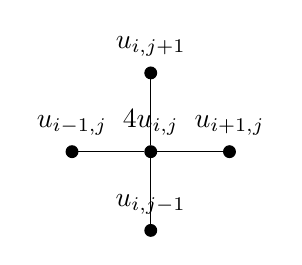
\begin{tikzpicture}
	\stencilpt{-1,0}{i-1}{$u_{i-1,j}$};
	\stencilpt{ 0,0}{i}  {$4 u_{i,j}$};
	\stencilpt{ 1,0}{i+1}{$u_{i+1,j}$};
	\stencilpt{0,-1}{j-1}{$u_{i,j-1}$};
	\stencilpt{0, 1}{j+1}{$u_{i,j+1}$};
	\draw 	(j-1) -- (i)
	(i)   -- (j+1)
	(i-1) -- (i)
	(i)   -- (i+1);
	\end{tikzpicture}}, i.e., for $i,j=2,\ldots,n-1$,
\begin{equation*}
\nabla^2_h u_{i,j} = \frac{4 u_{i,j} - u_{i-1,j} - u_{i,j-1} - u_{i+1,j} - u_{i,j+1} }{h^2} + O(h^2).
\end{equation*}
We can then express the the vector algebraic function whose zero approximates the solution to the minimization problem for~\eqref{eq:functional} as 
\begin{equation}\label{eq:zerotobe}
	F(\mathbf{u}) = \varepsilon^2 A \mathbf{u} - \mathbf{u} + \mathbf{u}^3 - \mathbf{f} = 0.
\end{equation}
Then, the (generic) Newton iteration for this problem reads as 
\begin{itemize}
	\item Given an initial guess $\mathbf{u}_0 = [1,1,\ldots,1]^T$,
	\item For $k=1,2,\ldots$ until convergence (or maximum allotted iterations)
	\begin{itemize}
		\item Solve for $J_F( \mathbf{u}_k ) \mathbf{d}_k = - F( \mathbf{u}_k )$,
		\item Update our guess $\mathbf{u}_{k+1} = \mathbf{u}_k + \lambda_k \mathbf{d}_k$.
	\end{itemize}
\end{itemize}
Where $J_F(\mathbf{u}) = F'(\mathbf{u})$ is the system Jacobian. The ``generality'' is inherent to a certain number of choices regarding the computation of the step--size $\lambda_k$, the update rate for the Jacobian, and so on. This part of the library has not been modified, so we refer back to \cite[Chapter~4]{kinsolguide}, and focus instead on the construction of the objects and the routines needed for launching the KINSOL module.

Before, entering into the details regarding the implementation, we compute also a closed form expression of the Jacobian $J_F(\mathbf{c})$ for~\eqref{eq:zerotobe}, that reads
\begin{equation}\label{eq:jacobian}
J_F(\mathbf{u}) = \varepsilon^2 A -I +3\operatorname{diag}(\mathbf{u}^2).
\end{equation}

As we have discussed in the general framework, the first step is to initialize the PSBLAS environment and to set the distribution of the data. In this case we are going to use also the interoperability between PSBLAS and MPI to use some native MPI functions, thus we recover also the MPI Communicator from the PSBLAS context,
\begin{lstlisting}[style=CStyle]
psb_i_t      ictxt;     /* PSBLAS Context            */
MPI_Comm     comm;      /* MPI Communicator          */
psb_i_t      np, iam;   /* Number of procs, proc id  */
ictxt = psb_c_init();
psb_c_info(ictxt,&iam,&np);
comm = MPI_Comm_f2c(ictxt);
\end{lstlisting}

The next step is then deciding the distribution of the data among the processes, this is analogous to what we have seen in the other examples, and can be achieved by
\begin{lstlisting}[style=CStyle]
psb_c_descriptor *cdh;  /* PSBLAS Descriptor         */
psb_l_t     n,m,nt,nr;
psb_i_t     nlr;

cdh = psb_c_new_descriptor();
psb_c_set_index_base(0);
m = ((psb_l_t) idim )*idim;
n = m;
nt = (m+np-1)/np;
nr = fmax(0,fmin(nt,m-(iam*nt)));
nt = nr;
MPI_Allreduce(MPI_IN_PLACE,&nt,1,MPI_LONG,MPI_SUM,comm);
if(nt != m){
 printf("%d Initialization error %ld %ld %ld\n",iam,nr,nt,m);
 psb_c_barrier(ictxt);
 psb_c_abort(ictxt);
 return(1);
}
if (info=psb_c_cdall_nl(nr, ictxt, cdh)!=0) {
 fprintf(stderr,"From cdall: %d\nBailing out\n",info);
 psb_c_abort(ictxt);
}
nlr = psb_c_cd_get_local_rows(cdh);
\end{lstlisting}
We are going again for a simple block distribution of the unknowns, in this case another feasible way of performing the data distribution would have been using the \lstinline[style=CStyle]|MPI_Cart_coords| MPI function to achieve a bi-dimensional distribution related to the grid.

The next step is then building the pieces needed to perform the computations of $F(\mathbf{u})$ in~\eqref{eq:zerotobe}. In this case the parts that is useful to have computed just one time and to be kept in memory are the matrix $\varepsilon^2 A$ and the forcing term $\mathbf{f}$. While we are at this, we observe also the the Jacobian in~\eqref{eq:jacobian} shares the same pattern of the $A$ matrix, thus we can also build at the same time the template for it. Moreover, since this is a test problem, we build also the true solution. We use the functions from Section~\ref{sec:nvector}, and Section~\ref{sec:sunmatrix} to initialize and allocate the space for the matrix.
\begin{lstlisting}[style=CStyle]
LAP = NULL;  /* The matrix epsilon^2 A */
LAP = SUNPSBLASMatrix(ictxt, cdh); 
J = NULL;    /* The prototype for the Jacobian */
J = SUNPSBLASMatrix(ictxt, cdh);
fvec = NULL; /* The forcing term f */
fvec = N_VNew_PSBLAS(ictxt, cdh);
\end{lstlisting}
We first compute some useful quantities, namely, the scaling,
\begin{lstlisting}[style=CStyle]
/* We loop over rows belonging to current process using our BLOCK data distribution.                             */
deltah   = ((psb_d_t) 1.0)/(idim+1);
sqdeltah = deltah*deltah;
deltah2  = ((psb_d_t) 2.0)*deltah;
sizes[0] = idim;
sizes[1] = idim;
\end{lstlisting}
then we query the communicator to discover what are the global indexes that we own,
\begin{lstlisting}[style=CStyle]
owned = SUNTRUE;
myidx = (psb_l_t *) malloc( sizeof(psb_l_t)*nlr );
psb_c_cd_get_global_indices(myidx,nlr,owned,cdh);
\end{lstlisting}
we build an auxiliary matrix consisting of one row at a time; just a
small matrix, the procedure might be extended to generate a group of rows per call
\begin{lstlisting}[style=CStyle]
val = (psb_d_t *) malloc( sizeof(psb_d_t)*20*nb );
irow = (psb_l_t *) malloc( sizeof(psb_l_t)*20*nb );
icol = (psb_l_t *) malloc( sizeof(psb_l_t)*20*nb );
\end{lstlisting}
Finally we launch the whole assembly procedure as
\begin{lstlisting}[style=CStyle]
psb_c_barrier(ictxt);
for(int ii = 0; ii < nlr; ii += nb){
	ib = fmin(nb,nlr-ii+1);
	localvecindex = (psb_l_t *) malloc( sizeof(psb_l_t)*ib );
	valj = (psb_d_t *) malloc( sizeof(psb_d_t)*ib );
	icoeff = 0;
	for(int kk = 0; kk < ib; kk++){
		i = ii + kk;
		glob_row = myidx[i]-1;              // Local Matrix Pointer
		psb_c_l_idx2ijk(ijk,glob_row,sizes,modes,base);
		x = (ijk[0]+1)*deltah;
		y = (ijk[1]+1)*deltah;
		
		zt[kk] = f(x,y,epsilon);
		ut[kk] = solution(x,y,epsilon);
		/* Internal point: build discretization                  */
		// term depending on   (x-1,y)
		val[icoeff] = -d(x,y,epsilon)/sqdeltah;
		if (ijk[0] == 0) {
			zt[kk] = g( (psb_d_t) 0, y )*(-val[icoeff]) + zt[kk];
		}else{
			ijktemp[0]   = ijk[0]-1;
			ijktemp[1]   = ijk[1];
			icol[icoeff] = psb_c_l_ijk2idx(ijktemp,sizes,modes,base);
			irow[icoeff] = glob_row;
			icoeff       = icoeff + 1;
		}
		// term depending on     (x,y-1)
		val[icoeff] = -d(x,y,epsilon)/sqdeltah;
		if (ijk[1] == 0) {
			zt[kk] = g(x,(psb_d_t) 0)*(-val[icoeff]) + zt[kk];
		}else{
			ijktemp[0]   = ijk[0];
			ijktemp[1]   = ijk[1]-1;
			icol[icoeff] = psb_c_l_ijk2idx(ijktemp,sizes,modes,base);
			irow[icoeff] = glob_row;
			icoeff       = icoeff + 1;
		}
		// term depending on     (x,y)
		val[icoeff]  = ( (psb_d_t) 2.0 )*(d(x,y,epsilon) + d(x,y,epsilon))/sqdeltah;
		icol[icoeff] = psb_c_l_ijk2idx(ijk,sizes,modes,base);
		irow[icoeff] = glob_row;
		icoeff       = icoeff + 1;
		//  term depending on     (x,y+1)
		val[icoeff] = -d(x,y,epsilon)/sqdeltah;
		if(ijk[1] == idim - 1){
			zt[kk] = g(x,(psb_d_t) 1.0)*(-val[icoeff]) + zt[kk];
		}else{
			ijktemp[0]   = ijk[0];
			ijktemp[1]   = ijk[1]+1;
			icol[icoeff] = psb_c_l_ijk2idx(ijktemp,sizes,modes,base);
			irow[icoeff] = glob_row;
			icoeff       = icoeff + 1;
		}
		// term depending on     (x+1,y)
		val[icoeff] = -d(x,y,epsilon)/sqdeltah;
		if(ijk[0] == idim - 1){
			zt[kk] = g((psb_d_t) 1.0,y)*(-val[icoeff]) + zt[kk];
		}else{
			ijktemp[0]   = ijk[0]+1;
			ijktemp[1]   = ijk[1];
			icol[icoeff] = psb_c_l_ijk2idx(ijktemp,sizes,modes,base);
			irow[icoeff] = glob_row;
			icoeff       = icoeff + 1;
		}
	}
	info = SUNMatIns_PSBLAS(icoeff,irow,icol,val,LAP);
	info = SUNMatIns_PSBLAS(icoeff,irow,icol,val,J);
	if(info != 0) printf("%d Error in SUNMatIns! %d\n",iam,info);
	icoeff = 0;
	for(int jj=ii; jj < ii+ib; jj++){
		localvecindex[icoeff] = myidx[jj]-1;
		valj[icoeff] = 1.0;
		icoeff++;
	}
	info = psb_c_dgeins(ib,localvecindex,zt,NV_PVEC_P(fvec),NV_DESCRIPTOR_P(fvec));
	if(info != 0) printf("%d Error in dgeins! %d\n",iam,info);
	info = psb_c_dgeins(ib,localvecindex,ut,NV_PVEC_P(utrue),NV_DESCRIPTOR_P(utrue));
	if(info != 0) printf("%d Error in dgeins! %d\n",iam,info);
	if(info != 0) printf("%d Error in SUNMatIns! %d\n",iam,info);
	free(localvecindex);
}
\end{lstlisting}
Now that the insert phase has been completed we need to assemble both the communicator, the two matrices, and the two vectors.
\begin{lstlisting}[style=CStyle]
psb_c_cdasb(cdh);
N_VAsb_PSBLAS(utrue);
N_VAsb_PSBLAS(fvec);
SUNMatAsb_PSBLAS(J);
SUNMatAsb_PSBLAS(LAP);
\end{lstlisting}
Before putting together the KINSOL solver we need
\begin{enumerate}
	\item the function computing $F(\mathbf{u})$,
	\item the function computing $J_F(\mathbf(u))$,
	\item an initial guess $\mathbf{u}$.
\end{enumerate}
For this case, as initial guess, we simply select the constant vector with all entries equal to one, namely
\begin{lstlisting}[style=CStyle]
u = NULL;
u = N_VNew_PSBLAS(ictxt, cdh);
N_VConst(1.0,u);
\end{lstlisting}
Then the function for $F(\mathbf{u})$ can be defined as
\begin{lstlisting}[style=CStyle]
static int funcprpr(N_Vector u, N_Vector fval, void *user_data){
struct user_data_for_f *input = user_data;
N_Vector cc;
cc = N_VNew_PSBLAS(NV_ICTXT_P(u),NV_DESCRIPTOR_P(u));
N_VAsb_PSBLAS(cc);
N_VAsb_PSBLAS(fval);
// cc <- u
N_VLinearSum( (psb_d_t) 1.0,u,(psb_d_t) 0.0,cc,cc);     
// F(u) = -epsilon^2*A*u - u -f + u^3
SUNMatMatvec_PSBLAS( *input->A, cc, fval );// fval <- Lap cc
N_VLinearSum_PSBLAS( (psb_d_t) -1.0, *input->f, (psb_d_t) 1.0, fval, fval); // fval = fval - f
N_VLinearSum_PSBLAS( (psb_d_t) -1.0, cc, (psb_d_t) 1.0, fval, fval); // fval = fval - cc     
N_VProd_PSBLAS(cc,u,cc); // cc^2 = cc.*u                      
N_VProd_PSBLAS(cc,u,cc); // cc^3 = u.*cc^2                    
// fval = fval - cc^3  
N_VLinearSum_PSBLAS( (psb_d_t) +1.0, cc, (psb_d_t) 1.0, fval, fval);        
N_VDestroy(cc);
return(0);
} 
\end{lstlisting}
where we are using the auxiliary structure \lstinline[style=CStyle]|user_data_for_f| to store the auxiliary data we need during the assembly, i.e.,
\begin{lstlisting}[style=CStyle]
struct user_data_for_f {
	SUNMatrix *A;
	N_Vector *f;
	psb_i_t sizes[2];
	psb_d_t sqdeltah;
	psb_d_t epsilon;
};
struct user_data_for_f user_data;/* User data for F,J */
/* We put the precomputed parts in the auxiliary data structure, this will be used to make both nonlinear function evaluations and Jacobian evaluations */
user_data.A = &LAP;
user_data.f = &fvec;
user_data.sizes[0] = sizes[0];
user_data.sizes[1] = sizes[1];
user_data.sqdeltah = sqdeltah;
user_data.epsilon  = epsilon;
\end{lstlisting}
In a similar way the routine of the Jacobian is a replica of the procedure we have used to compute $A$, in which we have changed the term on the diagonal, i.e.,
\begin{lstlisting}[style=CStyle]
static int jac(N_Vector yvec, N_Vector fvec, SUNMatrix J,
void *user_data, N_Vector tmp1, N_Vector tmp2)
{
	
	struct user_data_for_f *input = user_data;
	psb_l_t     *myidx,*irow,*icol,glob_row;
	psb_i_t      nlr,ib,icoeff,ijk[2],ijktemp[2],modes=2,base=0,i,iam,np,info;
	psb_d_t     *val,x,y, epsilon = input->epsilon, zt[nb];
	psb_d_t     sqdeltah = input->sqdeltah, deltah;
	psb_i_t     *sizes  =  input->sizes;
	psb_i_t     idim = sizes[0];
	bool        owned;
	deltah = sqrt(sqdeltah);
	
	// Who are we?
	psb_c_info(SM_ICTXT_P(J),&iam,&np);
	if(iam == 0){
		printf("\tBuilding a new Jacobian\n");
		printf("\tSize of the grid %d x %d\n",sizes[0],sizes[1]);
		printf("\tepsilon = %1.2e deltah = %1.2e\n",epsilon,sqdeltah);
	}
	SUNMatZero(J); // We put to zero the old Jacobian to reuse the structure
	
	nlr = psb_c_cd_get_local_rows(SM_DESCRIPTOR_P(J));
	owned = SUNTRUE;
	myidx = (psb_l_t *) malloc( sizeof(psb_l_t)*nlr );
	psb_c_cd_get_global_indices(myidx,nlr,owned,NV_DESCRIPTOR_P(yvec));
	
	/* we build an auxiliary matrix consisting of one row at a time; just a
	small matrix. might be extended to generate a bunch of rows per call. */
	val = (psb_d_t *) malloc( sizeof(psb_d_t)*20*nb );
	irow = (psb_l_t *) malloc( sizeof(psb_l_t)*20*nb );
	icol = (psb_l_t *) malloc( sizeof(psb_l_t)*20*nb );
	
	for(int ii = 0; ii < nlr; ii += nb){
		ib = fmin(nb,nlr-ii+1);
		icoeff = 0;
		for(int kk = 0; kk < ib; kk++){
			i = ii + kk;
			glob_row = myidx[i]-1;              // Local Matrix Pointer
			psb_c_l_idx2ijk(ijk,glob_row,sizes,modes,base);
			x = (ijk[0]+1)*deltah;
			y = (ijk[1]+1)*deltah;
			
			zt[kk] = f(x,y,epsilon);
			/* Internal point: build discretization                  */
			// term depending on   (x-1,y)
			val[icoeff] = -d(x,y,epsilon)/sqdeltah;
			if (ijk[0] == 0) {
				zt[kk] = g( (psb_d_t) 0, y )*(-val[icoeff]) + zt[kk];
			}else{
				ijktemp[0]   = ijk[0]-1;
				ijktemp[1]   = ijk[1];
				icol[icoeff] = psb_c_l_ijk2idx(ijktemp,sizes,modes,base);
				irow[icoeff] = glob_row;
				icoeff       = icoeff + 1;
			}
			// term depending on     (x,y-1)
			val[icoeff] = -d(x,y,epsilon)/sqdeltah;
			if (ijk[1] == 0) {
				zt[kk] = g(x,(psb_d_t) 0)*(-val[icoeff]) + zt[kk];
			}else{
				ijktemp[0]   = ijk[0];
				ijktemp[1]   = ijk[1]-1;
				icol[icoeff] = psb_c_l_ijk2idx(ijktemp,sizes,modes,base);
				irow[icoeff] = glob_row;
				icoeff       = icoeff + 1;
			}
\end{lstlisting}
Here we have the change with respect to $A$, and we use the elements of the current solution
\begin{lstlisting}[style=CStyle]
			// term depending on     (x,y)
			val[icoeff]  = ( (psb_d_t) 2.0 )*(d(x,y,epsilon) + d(x,y,epsilon))/sqdeltah
			-((psb_d_t) 1.0) + ((psb_d_t) 3.0)*pow((N_VGetArrayPointer_PSBLAS(yvec))[i],2.0);
			icol[icoeff] = psb_c_l_ijk2idx(ijk,sizes,modes,base);
			irow[icoeff] = glob_row;
			icoeff       = icoeff + 1;
			//  term depending on     (x,y+1)
			val[icoeff] = -d(x,y,epsilon)/sqdeltah;
			if(ijk[1] == idim - 1){
				zt[kk] = g(x,(psb_d_t) 1.0)*(-val[icoeff]) + zt[kk];
			}else{
				ijktemp[0]   = ijk[0];
				ijktemp[1]   = ijk[1]+1;
				icol[icoeff] = psb_c_l_ijk2idx(ijktemp,sizes,modes,base);
				irow[icoeff] = glob_row;
				icoeff       = icoeff + 1;
			}
			// term depending on     (x+1,y)
			val[icoeff] = -d(x,y,epsilon)/sqdeltah;
			if(ijk[0] == idim - 1){
				zt[kk] = g((psb_d_t) 1.0,y)*(-val[icoeff]) + zt[kk];
			}else{
				ijktemp[0]   = ijk[0]+1;
				ijktemp[1]   = ijk[1];
				icol[icoeff] = psb_c_l_ijk2idx(ijktemp,sizes,modes,base);
				irow[icoeff] = glob_row;
				icoeff       = icoeff + 1;
			}
		}
		info = SUNMatIns_PSBLAS(icoeff,irow,icol,val,J);
		if(info != 0) printf("%d Error in SUNMatIns! %d\n",iam,info);
	}
	
	SUNMatAsb_PSBLAS(J);
	if(iam == 0){
		printf("\tBuilding phase completed\n");
	}
	
	/* Free the Memory for the Auxiliary Array */
	free(val);
	free(irow);
	free(icol);
	free(myidx);
	
	return(0);
}
\end{lstlisting}

Now we have almost all the bits and pieces on the PSBLAS side needed to the define our KINSOL solver, the last thing we need is a vector of constraints than need to be enforced on the Newton iteration, since in this case we have no constraint to enforce this is simply a constant vector of zeros, i.e.,
\begin{lstlisting}[style=CStyle]
constraints = NULL;
constraints = N_VNew_PSBLAS(ictxt, cdh);
N_VConst(0.0,constraints);
\end{lstlisting}
and then we define the nonlinear solver as 
\begin{lstlisting}[style=CStyle]
/* Call KINCreate/KINInit to initialize KINSOL:
A pointer to KINSOL problem memory is returned and stored in kmem. */
kmem = KINCreate();
info = KINInit(kmem, funcprpr, u);
info = KINSetNumMaxIters(kmem, newtonmaxit);
info = KINSetPrintLevel(kmem, 0);
info = KINSetUserData(kmem, &user_data);
info = KINSetConstraints(kmem, constraints);
info = KINSetFuncNormTol(kmem, fnormtol);
info = KINSetScaledStepTol(kmem, scsteptol);
/* We no longer need the constraints vector since KINSetConstraints creates a private copy for KINSOL to use. */
N_VDestroy(constraints);
\end{lstlisting}
We refer to the guide~\cite{kinsolguide} for the meaning of the different options. Now we need to tell KINSOL how we would like our linear systems with the Jacobian matrix to be solved. We are using a matrix-based approach, so we need to exploit the solver we have introduced in Section~\ref{sec:sunlinsol}. Therefore, we build an instance of a PSBLAS solver with a ML preconditioner by doing
\begin{lstlisting}[style=CStyle]
/* We create now the linear systes solver */
psb_c_DefaultSolverOptions(&options);
options.eps    = tol;
options.itmax  = itmax;
options.irst   = irst;
options.itrace = 1;
options.istop  = istop;
/* Create PSBLAS/MLD2P4 linear solver */
LS = SUNLinSol_PSBLAS(options, methd, ptype, ictxt);
\end{lstlisting}
Then we set the option for the Multigrid preconditioner as 
\begin{lstlisting}[style=CStyle]
SUNLinSolInitialize_PSBLAS(LS);
info = SUNLinSolSeti_PSBLAS(LS,"SMOOTHER_SWEEPS",2);
info = SUNLinSolSeti_PSBLAS(LS,"SUB_FILLIN",1);
info = SUNLinSolSetc_PSBLAS(LS,"COARSE_SOLVE","BJAC");
info = SUNLinSolSetc_PSBLAS(LS,"COARSE_SUBSOLVE","ILU");
\end{lstlisting}
We can then the PSBLAS linear solver (together with its preconditioner) to KINSOL by doing
\begin{lstlisting}[style=CStyle]
info = KINSetLinearSolver(kmem, LS, J);
info = KINSetJacFn(kmem,jac);
info = KINSetEtaForm(kmem,KIN_ETACONSTANT);
info = KINSetEtaConstValue(kmem,options.eps);
\end{lstlisting}
Now the setup phase is completed, and we have only to call the solver on our problem. This is achieved by doing
\begin{lstlisting}[style=CStyle]
info = KINSol(kmem,/* KINSol memory block                  */
	u,             /* initial guess on input/solution vector */
	globalstrategy,/* global strategy choice                 */
	sc,    /* scaling vector for the variable u              */
	sc);   /* scaling vector for function values fval        */
\end{lstlisting}
where the scaling vector is simply
\begin{lstlisting}[style=CStyle]
sc = NULL;
sc = N_VNew_PSBLAS(ictxt, cdh);
N_VConst(1e-4*sqdeltah,sc);
\end{lstlisting}
\marginlabel{
	\includegraphics[width=\leftmarginwidth]{ginzburglandausolution.pdf}
	{\flushleft Solution of~\eqref{eq:zerotobe} for a $60\times 60$ grid.}
}At the end of this call the vector $\mathbf{u}$ will contain our approximate solution, on the left we have given a plot of the solution of the point-wise difference with the true solution for a $60\times 60$ grid.

The complete code for running the example, and having the possibilities of changing both the parameters of the solvers and of the problems, is contained in \texttt{examples/kinsol/psblas}.


\appendix

\section{Matrix assembly routine}
The following routine loops through the local entries of the communicator allocate in Listing~\ref{lst:example_of_allocation}, and uses the \texttt{SUNMatIns\_PSBLAS} routine to insert the entries in the sparse matrix. The auxiliary functions $\{a_{i},b_i,g\}_{i=1}^3$ take care of the coefficient functions in~\eqref{eq:boundaryproblem}.
\begin{lstlisting}[style=CStyle,caption="Allocation routine for the discrete boundary value problem~\eqref{eq:boundaryproblem}.",label=lst:allocationroutine]
psb_i_t matgen(psb_i_t ictxt, psb_i_t nl, psb_i_t idim, psb_l_t vl[],SUNMatrix A)
{
psb_i_t iam, np;
psb_l_t ix, iy, iz, el,glob_row;
psb_i_t i, k, info;
double x, y, z, deltah, sqdeltah, deltah2;
double val[10*NBMAX], zt[NBMAX];
psb_l_t irow[10*NBMAX], icol[10*NBMAX];

info = 0;
psb_c_info(ictxt,&iam,&np);
deltah = (double) 1.0/(idim+1);
sqdeltah = deltah*deltah;
deltah2  = 2.0* deltah;
psb_c_set_index_base(0);
for (i=0; i<nl;  i++) {
glob_row=vl[i];
el=0;
ix = glob_row/(idim*idim);
iy = (glob_row-ix*idim*idim)/idim;
iz = glob_row-ix*idim*idim-iy*idim;
x=(ix+1)*deltah;
y=(iy+1)*deltah;
z=(iz+1)*deltah;
zt[0] = 0.0;
/*  internal point: build discretization */
/*  term depending on   (x-1,y,z)        */
val[el] = -a1(x,y,z)/sqdeltah-b1(x,y,z)/deltah2;
if (ix==0) {
zt[0] += g(0.0,y,z)*(-val[el]);
} else {
icol[el]=(ix-1)*idim*idim+(iy)*idim+(iz);
el=el+1;
}
/*  term depending on     (x,y-1,z) */
val[el]  = -a2(x,y,z)/sqdeltah-b2(x,y,z)/deltah2;
if (iy==0) {
zt[0] += g(x,0.0,z)*(-val[el]);
} else {
icol[el]=(ix)*idim*idim+(iy-1)*idim+(iz);
el=el+1;
}
/* term depending on     (x,y,z-1)*/
val[el]=-a3(x,y,z)/sqdeltah-b3(x,y,z)/deltah2;
if (iz==0) {
zt[0] += g(x,y,0.0)*(-val[el]);
} else {
icol[el]=(ix)*idim*idim+(iy)*idim+(iz-1);
el=el+1;
}
/* term depending on     (x,y,z)*/
val[el]=2.0*(a1(x,y,z)+a2(x,y,z)+a3(x,y,z))/sqdeltah + c(x,y,z);
icol[el]=(ix)*idim*idim+(iy)*idim+(iz);
el=el+1;
/*  term depending on     (x,y,z+1) */
val[el] = -a3(x,y,z)/sqdeltah+b3(x,y,z)/deltah2;
if (iz==idim-1) {
zt[0] += g(x,y,1.0)*(-val[el]);
} else {
icol[el]=(ix)*idim*idim+(iy)*idim+(iz+1);
el=el+1;
}
/* term depending on     (x,y+1,z) */
val[el] = -a2(x,y,z)/sqdeltah+b2(x,y,z)/deltah2;
if (iy==idim-1) {
zt[0] += g(x,1.0,z)*(-val[el]);
} else {
icol[el]=(ix)*idim*idim+(iy+1)*idim+(iz);
el=el+1;
}
/*  term depending on     (x+1,y,z) */
val[el] = -a1(x,y,z)/sqdeltah+b1(x,y,z)/deltah2;
if (ix==idim-1) {
zt[0] += g(1.0,y,z)*(-val[el]);
} else {
icol[el]=(ix+1)*idim*idim+(iy)*idim+(iz);
el=el+1;
}
for (k=0; k<el; k++) irow[k]=glob_row;
if ((info=SUNMatIns_PSBLAS(el,irow,icol,val,A))!=0)
fprintf(stderr,"From psb_c_dspins: %d\n",info);
}

return(info);
}
\end{lstlisting}

Observe that to speed-up the insertion procedure we are collecting together a certain number of rows to be inserted, specifically \texttt{10*NBMAX} for a defined value of NBMAX. It is clearly possible to execute one call for
each nonzero coefficient, however this would have a substantial computational
overhead. Therefore packing a ``certain amount of data'' (\texttt{10*NBMAX}) into each call
to the insertion routine is advisable. The best performing value of \texttt{NBMAX} depends on both the architecture of the computer being used and
on the problem structure.

\printbibliography[heading=bibintoc]

\end{document} 